\documentclass[a4paper, twocolumn, 10pt]{article}

%Paquetes idioma
\usepackage[utf8]{inputenc}
\usepackage[spanish]{babel}

%Paquetes matemáticas
\usepackage{amsmath}
\usepackage{amsfonts}
\usepackage{amssymb}

%Paquetes variados y organización
\usepackage{graphicx}
\usepackage[left=2cm,right=2cm,top=2cm,bottom=2cm]{geometry}
\usepackage{multicol}
\usepackage{float}
\usepackage{multirow}
\usepackage{subfigure}
\usepackage{cite}
\usepackage{stfloats}
\usepackage{array}
%Paquetes matemáticas
\usepackage{amsmath}
\usepackage{amsfonts}
\usepackage{amssymb}
\usepackage{listings}
\usepackage{color}
\usepackage{graphicx} % figuras
\usepackage{subfigure} % subfiguras
\usepackage{paralist} % Used for the compactitem environment which makes bullet points with less space between them
\usepackage[none]{hyphenat}
\usepackage{afterpage}


%Paquetes variados y organización
\usepackage{graphicx}
\usepackage[left=2cm,right=2cm,top=2cm,bottom=2cm]{geometry}
\usepackage{multicol}
\usepackage{float}
\usepackage{multirow}
\usepackage{subfigure}
\usepackage{cite}
\usepackage{stfloats}
\usepackage{array}

\usepackage{fancyhdr}
\usepackage{fontspec}
\pagestyle{fancy} % seleccionamos un estilo
\usepackage{subfig}

\usepackage[maxbibnames=99, sorting=none, backend=bibtex]{biblatex}
\addbibresource{bibio.bib}

\usepackage{fancyhdr}
\usepackage{graphicx}


\rhead{\begin{picture}(0,0) \put(-57,0){
\includegraphics[width=20mm]{./uis}} \end{picture}}
\chead{ Metalentes y metamateriales en insectos \vspace{0.1cm}}
\renewcommand{\headrulewidth}{0.5pt}



%Datos del informe
\title{\textbf{ Propiedades ópticas de un metalente presentes en el fenómeno de iridiscencia en algunos insectos}} 
\author{Jorge Andrés Quintero Graut$^1$, Angie Milena Sanchez$^1$\\ \textit{Universidad Industrial de Santander$^1$}}

\begin{document}
\sloppy 
\twocolumn[
\begin{@twocolumnfalse}
\maketitle
\begin{abstract}

%\noindent{La partícula con carga eléctrica en un campo magnético describe un movimiento circular uniforme, gracias a que la fuerza magnética es  perpendicular a la velocidad de dicho cuerpo.  Para obtener la carga especifica del electrón se realizó la toma de datos de corriente para cada valor de potencial, además de la calibración de campo magnético, fue necesario hallar la pendiente de cada gráfico y así poder hacer uso de la ecuación de la carga especifica del electrón, para la cual se obtuvo un valor experimental de 5.0133$\times10^{11}$ [c/kg]}
\noindent Este trabajo consistió en bucar una forma alternativa de evidenciar experimentalmente algunas propiedades ópticas que poseen los metalentes, tales como él indice de refracción ($n$), permitividad ($\epsilon$) y permeabilidad ($\mu$) menores a cero, y las implicaciones que trae consigo estos efectos. Para ello se observó y comparó la microestructura morfológica de algunos invertebrados, con la estructura que posee un metalente. De esta forma se pudo corroborar que dependiendo de la geometría presente en el sistema a estudiar fue posible notar que en una de las especies escogidas puede hacer un acercamiento a lo que es un metalente, algunos, por otro lado aplicaría para el concepto de metamaterial.

\begin{center}\rule{0.9\textwidth}{0.1mm} \end{center}
\end{abstract}
\end{@twocolumnfalse}
]
%\section*{Resumen}

\section*{Introducción}

\noindent Los metamateriales se conocen como aquellos materiales artificiales creados a conveniencia humana para cumplir con ciertas propiedades de tipo ópticas. Estas propiedades pueden variar debido a su composición química y/o también por la organización de la nano estructura presente en determinado material. Por otro lado, tener un metamaterial a disposición en Colombia presenta complicaciones, no obstante, en este proyecto se pretende mostrar posibles propiedades o comportamientos de metamateriales en algunos insectos en la naturaleza tales como escarabajos, abejas y cigarras, animales que poseean iridicencia en su morfología. De esta manera se logra tener un acercamiento experimental en la presente área de investigación. Cabe resaltar que el formalismo y modelamiento tanto físico como matemático para estos materiales varía considerablemente en comparación con los materiales naturales.

\section*{Objetivos}

\begin{itemize}
    \item Mostrar el fundamento teórico de las metalentes.
    \item Explicar el fenómeno de la iridiscencia en diferentes insectos a partir de las características que presentan los metamateriales
\end{itemize}

\section*{Fundamentos teóricos}


Para un material natural, la ecuación de dispersión viene dada por:

\begin{equation}
    \textbf{k}^2 = \frac{\omega^2}{c^2}n^2
\end{equation}

donde $k$ representa el vector de onda, $\omega$ la frecuencia angular, y $c$ la velocidad de la luz. El índice de refracción n está determinado por el complejo, las propiedades del material de frecuencia-dependientes permiten ε y la permeabilidad $\mu$.
En ese orden de ideas se puede escribir:

\begin{equation}
    n^2 = \epsilon\mu
\end{equation}

si se asume pérdidas insignificantes en los materriales y tomando $n$, $\mu$, y $\epsilon$ como números reales. Comenzando con las ecuaciones de Maxwell para una onda plana monocromática:

\begin{equation}
    \vec{k}*\vec{E} = \frac{w}{c}\mu\vec{H}
\end{equation}
Análogamente:


\begin{equation}
    \vec{k}*\vec{H} =- \frac{w}{c}\epsilon\vec{E}
\end{equation}



\subsection*{Refración negativa}

Una propiedad característica de ciertos metamateriales es que poseen un índice de refración negativo; aquellos que no lo poseen, modifican la fase del haz incidente por medio de una serie de rendijas semejantes a un iterferómetro de young.

\begin{figure}[H]
    \centering
    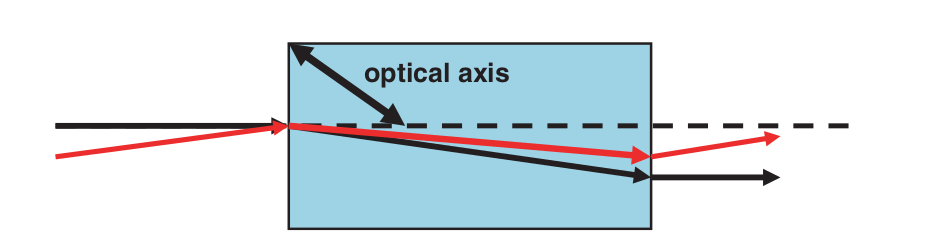
\includegraphics[width = 0.5\textwidth]{indice.png}
    \caption{ESquematización para los casos con índice de refración negativo y positivo.}
    \label{tipos}
\end{figure}

No obstanate, aquellos que sí poseen dicho índice de refracción se rigen bajo el siguiente formalismo:

Iniciando por las ecuaciones de maxwell, las realciones de dispersion de la lente a lo largo del eje $z$ viene dado por:


%kkkkkkkkkkkkkk eq
\begin{equation}
    k_z = \sqrt{\frac{\omega^2}{c^2}-k^2_x-k^2_y}
\end{equation}
donde:

\begin{equation*}
    \frac{\omega^}{c^2} > k^2_x+k^2_y
\end{equation*}
 
 y también:
 
 \begin{equation}
    k_z = i\sqrt{\frac{\omega^2}{c^2}+k^2_x-k^2_y}
\end{equation}
donde:

\begin{equation*}
    \frac{\omega^}{c^2} < k^2_x+k^2_y.
\end{equation*}

Teniendo en cuenta que la Ec. 3 representa ondas de propagación, mientras que la Ec. 4 representa ondas evanescentes que tienen un $\textbf{k}_z$ puramente imaginario . La permeabilidad, y el índice refractivo todos iguales a $-1$, con las condiciones de límite apropiadas para el espacio libre circundante, podemos resolver para la transmisión $T$:

\begin{equation}
    T  = e^{ik_zd_s}
\end{equation}

\noindent para las polarizaciones perpendiculares ($s$) y paralelas ($p$), donde d s es el espesor de la losa. La ecuación anterior es notable porque implica amplificación de ondas evanescentes. Sin embargo, además de requerir propiedades materiales que no existen en la naturaleza, este resultado sólo se obtiene en las condiciones de pérdida insignificante y buen ajuste de impedancia, y por lo tanto todavía no se ha realizado experimentalmente.

\noindent La ecuación 1 representa la propagación de las ondas y la ecuación 2 representa las ondas envanecentes.
Ahora, para un medio anisotrópico se considerará Consideremos un caso de refracción de la luz en la interfaz de dos medios uniformes, como se muestra en la figura. Se supone que los medios tienen Tensores de permitividad anisotrópica ε L y ε R, ambos con simetría uniaxial:

\begin{figure}[H]
    \centering
    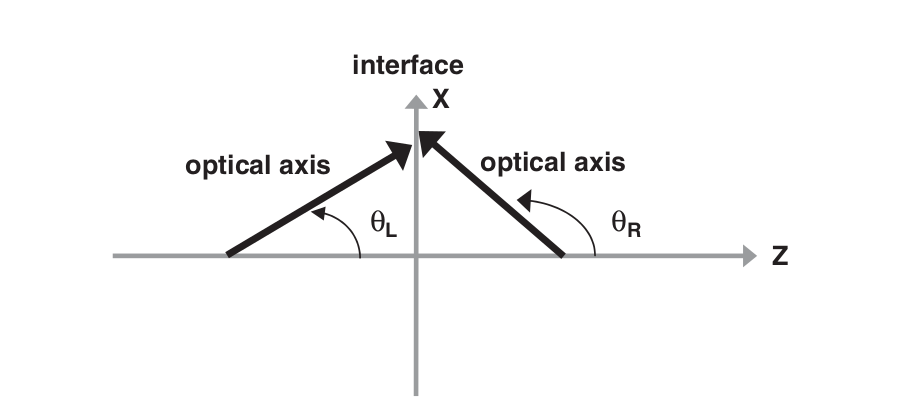
\includegraphics[width= 0.4\textwidth]{angulo.png}
    \caption{representación gráfica para indice de refracción en dos medios}
    \label{metasuperficie}
\end{figure}

\noindent Ahora, para la permeabilidad isotrópica, $\mu$ L y $\mu$ R, donde L y R denotan la mano izquierda y lado derecho, respectivamente. Se supone que sus ejes de simetría mienten
en el mismo plano que el plano de incidencia, que también es perpendicular a
la interfaz, pero puede inclinarse en cualquier ángulo con respecto a
interfaz normal.

Más bien discusiones generalizadas para el problema de reflexión-refracción asociado
con la interfaz definida, se han dado en la literatura para el
situación de ε 1 y ε 3 ambos positivos. Para una ola ordinaria con
campo eléctrico E polarizado en la dirección y, es decir, perpendicular al plano
de incidencia (una onda TE), el problema es equivalente a un caso isotrópico con
diferentes constantes dieléctricas ε L1 y ε R
1 para el lado izquierdo y derecho.
Es el reflejo y la refracción de la onda extraordinaria o polarizada H,
es decir, con E polarizada en el plano x – z (una onda TM), eso generalmente ha sido
resultó ser más interesante Para las ondas polarizadas E y H, la dispersión
Las relaciones se dan a continuación para los dos sistemas de coordenadas:

\begin{figure}[H]
    \centering
    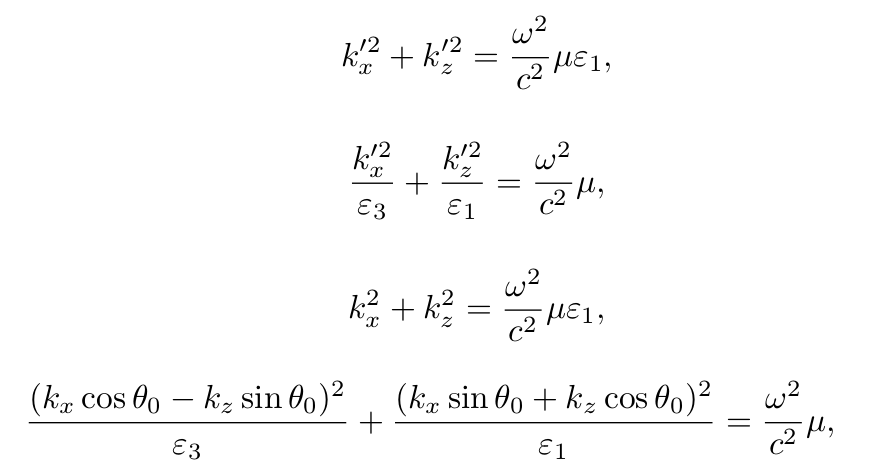
\includegraphics[width= 0.5\textwidth]{yaaaa.png}
    \caption{Relaciones de dispersión}
    \label{metasuperficie}
\end{figure}

\section{\textbf{Una revisión histórica}}

\noindent El papel básico de los componentes ópticos como lentes o prismas es dar forma a los frentes de onda entrantes. En los últimos años se han introducido y demostrado varios componentes ópticos planos con un espesor óptico en el orden de la longitud de onda. En contraste con la óptica a granel, donde la fase es modulada por una variación continua del espesor óptico, la óptica plana restringe la modulación a su mínimo, 2$ lambda$ , envolviendo el bulto - módulo de fase óptica 2 $ \lambda$ para una longitud de onda de diseño nominal $ \lambda$\\
\noindent Los metalentes combinan dos enfoques principales (emisión de ondas y antena), poe ello, es apropiado comenzar con el lente de retardo estudiado durante la segunda guerra mundial por Kock, quien fabricó lentes difractivas de microondas en dieléctricos artificiales de alto índice efectivos obtenidos por dopaje de láminas de espuma de poliestireno con insertos metálicos de sublongitud, i.e. antenas. Se logró una drástica reducción de peso con medio resonante de longitud de onda, pero se logró una operación de frecuencia más amplia con incluso ligeramente más pequeños inserciones de resonancia apagado.\\

\noindent La extensión a longitudes de onda más cortas, no ocurrió hasta mucho más recientemente. Investigadores en Erlangen y en el MIT ,fueron los primeros en proponer el seguimiento de la fase de los materiales artificiales de índice clasificados en el infrarrojo, y luego en el dominio visible por un (relativamente) cambio local lento del perfil de las rejillas de longitud de subonda alta. Las primeras demostraciones experimentales de rejillas de reflexión y un espejo cilíndrico se realizaron a $ \lambda = 10.6$ $\mu m$ con ranuras metálicas de anchuras graduadas.\\

\noindent Las demostraciones iniciales de dieléctricos artificiales de índice efectivo graduado fabricados para frecuencias visibles por grabado de películas de cuarzo, vidrio y polímero fueron decepcionantes, con eficiencias de difracción medidas menores que las de los componentes de échelette. En ese momento, el diseño asumía principalmente un gradiente de índice efectivo "adiabático", la analogía entre rejillas de longitud de subonda local y dieléctricas artificiales no se entendía correctamente, y el modelado era difícil. También es importante destacar que las necesidades combinadas de espaciado de la longitud de subonda y la fase de 2$ \pi$ de excursión condujeron a proporciones de aspecto difíciles de fabricar con los materiales y las tecnologías de modelado implementadas.

\noindent Nuevas perspectivas abiertas por la fabricación de componentes dieléctricos artificiales graduados en materiales de alto índice. Para el funcionamiento en lo visible, Tio 2 parecía ser el material transparente más adecuado. La Figura 4 resume los principales resultados, que se obtuvieron para una serie de rejillas con ángulo de desviación creciente para el funcionamiento en la línea láser con longitud de ona $ \lambda = 633$ nm.

\noindent La anchura más pequeña del conjunto de estas nanoestructuras es de 490 nm, y el espaciado de pilares utilizado para probar la fase es de 272 nm. Las rejillas, llamadas componentes binarios "blazed" de los autores, ya que introducen un nuevo tipo de componentes blazed derivados del enmascaramiento binario, fueron fabricadas por e directo - escritura de haz, despegue y grabado de iones reactivos asistidos químicamente utilizando un proceso detallado. Sorprendentemente, se observaron eficiencias que superaban los componentes de la échelette hegemónica para los tintes Gra altamente dispersivos correspondientes a grandes ángulos de desviación . El mismo concepto se aplica a las lentes: por primera vez, se podría prever la aplicación de lentes eficientes con NA alta, eliminando la primera limitación de las lentes de difracción échelette.
De hecho, esa demostración fue seguida inmediatamente por la fabricación de una lente de eje de $ 20 Circ$ apagado operando a $ lambda = 850$ nm con una vertical - superficie de la cavidad que emite láser para su posible aplicación a las interconexiones ópticas, vea la imagen SEM mostrada en Fig . 3 c. El objetivo tenía un NA o f 0.25 pero desde el fue diseñado para una operación de 20° fuera del eje, la zona de Fresnel anchos eran todos más pequeños que 9 $ \lambda$ . H alf de la abertura se compuso de zonas con anchuras menores a 3 $ \lambda$ , correspondiendo a un NA mucho más grande para un objetivo del eje. Aún así, la eficiencia medida, incluyendo las reflexiones de Fresnel, alcanza un impresionante 80\%.



\begin{figure}[H]
    \centering
    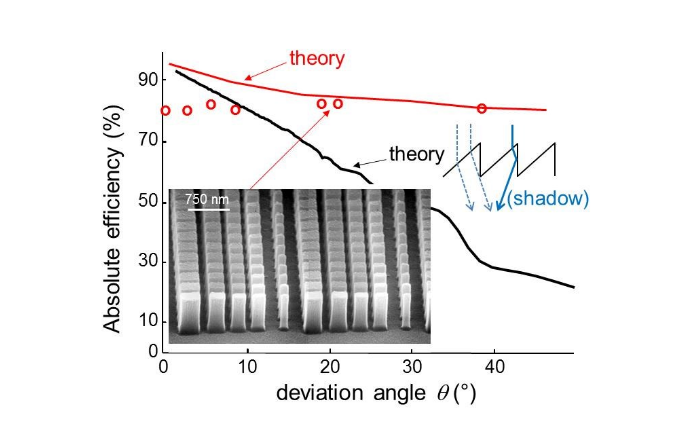
\includegraphics[width= 0.4\textwidth]{nano.png}
    \caption{ rejillas binarias brillantes golpean a sus contrapartes de échelette con respecto a la eficiencia \cite{li2019metalens}}
    \label{metasuperficie}
\end{figure}

\begin{figure}[H]
    \centering
    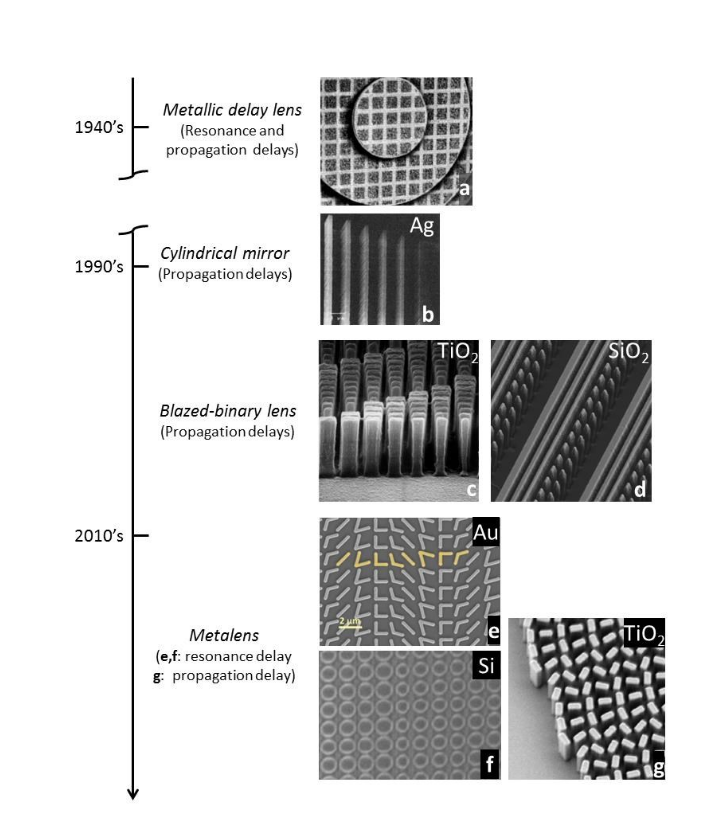
\includegraphics[width= 0.5\textwidth]{fechas.png}
    \caption{ Evolución histórica de los metalentes \cite{li2019metalens}}
    \label{metasuperficie}
\end{figure}

Para grandes ángulos de desviación, el ángulo del prisma en cada período de échelette es tan grande como para proyectar sombra sobre los vecinos, desperdiciando luz en órdenes espurios, como se ilustra en el derecho - lado de la mano de la Fig. 2 para la incidencia normal e. El efecto empeora en el ángulo de desviación grande y en la incidencia oblicua, como el impacto relativo de la zona de sombra en la difracción aumenta. En contraste, para los elementos difractivos binarios de alto - índice blanqueado - cada pilar se comporta como una guía de onda monomodo independiente que confina la luz en toda la estructura.



\subsection*{Definición de metalente}

\noindent La difracción de la luz impone un importante límite para todo sistema formador de imágenes. Este límite consiste en que dos objetos son distinguibles uno de otro a una larga distancia, si y solo si entre ellos las distancia de separación es más pequeña que la mitad de la longitud de onda de la luz usada para observarlos\cite{liu2017plasmonics}. Esto se evidencia en los microscópios fabrocados con lentes convencionales, en donde no se pueden distingir dos objetos si se encuentran a una distancia $d=\frac{\lambda}{2 N_a}$, siendo $\lambda$ la longitud de onda de la luz usada para realizar a observación y $N_a$ la apertura de la lente.\\


\noindent Los metalentes son lentes fabricados en base a metamateriales, los cuales permiten distinguir objetos que están separados una distancia menor a $ \sim \lambda/2$, es decir,las metalentes sobrepasan el límite impuesto por la difracción en lentes convencionales. El indice de refracción negativo sumado con los mecanismos de compensación de fase, permiten que los metamateriales puedan ser usados para la fabricación de lentes.\\

\noindent Estos lentes permiten obtener información de objetos de forma bien detallada en el campo lejano y magnificar las ondas evanescentes, que son ondas que no se propagan en la dirección normal de material, lograndose obtener información más detallada de la superficie. Por lo tanto, esta clase de lentes son consideradas lentes perfectas. Son capaces de enfocar la luz con muy alta resolución y disminuir las aberraciones opticas de forma considerable. Sus estructuras basadas en arreglos de diferentes materiales a escalas nanométricas, hacen posible la construcción de lentes muy pequeños.


\noindent Generalmente están formados por matamateriales plasmónicos y arrelos del tipo metal-dielectrico. Están diseñados de tal manera que se pueda realizar la trasnformada de Fourier al la luz que pase a través de ellos, a partir de mecanismos de compensación de la fase en la superficie del lente. Los arreglos se pueden realizar de forma períodica o no períódica. Algunos ejemplos de estos arreglos se ven en la figura \ref{metasuperficie}.


\noindent La luz al pasar del aire al metamarerial, se forma un cambio en su frecuencua espacial. La alta frecuencia espacial dentro de un metamaterial no puede trasmitirse al aire debido a la reflexxión total interna. Por lo tanto siempre es necesario un mecanismo pasa convertir ondas de alta frecuencia espacial a ondas de baja frecuencia espacial y viceversa.

\begin{figure}[H]
    \centering
    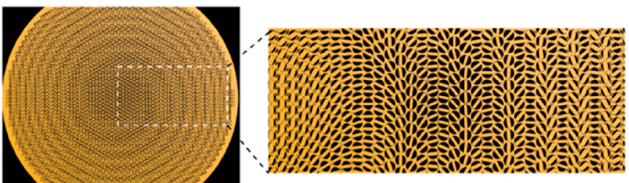
\includegraphics[width= 0.4\textwidth]{imagenarreglo.png}
    \caption{Metasuperficie diseñada como metalente. Imagen tomada de referencia \cite{li2019metalens}}
    \label{metasuperficie}
\end{figure}

\subsection*{Metalentes delgadas}

\subsection*{Tipos de metalentes.}


Las metalentes se pueden clasificar según su mecanismo de acople bidireccional de la luz. Estos son el PWC(PLasmonic waveguide coupler) y los metalentes fabricadas con base a cambios en el indice de refracción GRIN.

\subsubsection*{Cambiando la forma de la interfase aire-metamaterial}

Una manera de que se realice el acople bidireccional es por medio de una superficie hiperbólica en la interfase aire-metamaterial. Esto es debido a que la difracción hiperbólica produce un cambio de bajos a altos vectores de onda y la necesaria compensación e la fase.

\subsubsection*{Plasmonic Waveguide coupler(PWC)}

Están compuestos de arreglos no periódicos de subarreglos de orden metal-aislante-guia de onda metálica, para fomar la metasuperficie de la lente. De forma más precisa, luz que se propaga en el aire, pasa por la metasuperficie y se sigue propagando por el metamaterial. La metasuperficie se encarga que en el  medio metamaterial los frentes de onda incidentes dejen de ser planos, dedido a la condición de fase impuesta por  la interfase PWC. Esta metasuperficie enfoca las sublongitudes\cite{lu2012hyperlenses}.

\subsubsection*{Fabricados con en base a metamateriales GRIN}

Para modular el cambio de bajas frecuencias a altas frecuencias, se diseñan metamateriales donde le indice de refracción cambia en todo el espacio comprendido el metamaterial. Estas variaciones permiten que la luz pueda ser enforcada en un punto.


\begin{figure*}[h!]
    \centering
    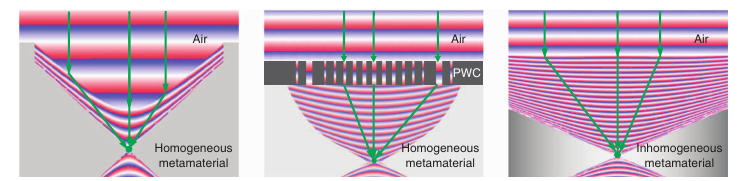
\includegraphics[width = 0.8\textwidth]{metalentes3.png}
    \caption{Tipos de metalentes según el mecanismo de acomple bidireccional: con una interfase aire-metamaterial hiperbólica(izquierda), con una interface PWC (centro) y un metamaterial GRIN (Derecha)}
    \label{tipos}
\end{figure*}

\subsubsection*{Fenómeno de Iridiscencia}


\noindent La iridiscencia se conoce como un fenómeno óptico  que poseen ciertas superficies en las cuales el tono de la luz varía de acuerdo al ángulo de incidencia de la luz (variación en la longitud de onda) sobre la superficie observada. La iridiscencia es causada por múltiples reflexiones de la luz (independientemente si es un metematerial o no) en diversas superficies semitransparentes, donde los subsecuentes cambios de fase e interferencia de las reflexiones modulan la luz por la amplificación o atenuación de las diferentes longitudes de onda. La iridiscencia es muy común en la naturaleza, se puede notar experimentalmente en insectos, aves y peces, e incluso en ciertas especies de plantas.

\noindent Si las longitudes de onda de los haces reflejados se encuentran en fase, se verá evidenciado el fenómeno de interferencia constructiva produciendo así, estos colores iridiscentes. Por el contrario si los dos rayos de luz que se reflejan tienen longitudes de onda en desafse, la intensidad de la luz de uno de los haces se verá opacada por el otro. Como las condiciones de interferencia dependen de la longitud de onda, la intensidad de luz reflejada por una película dada varía considerablemente con la longitud de onda. Ello produce los efectos de color de iridiscencia cuando se ilumina la película con luz blanca.\ref{iris}




\section{Metodología}

\noindent Para llevar a cabo esta práctica, fue necesario recurrir al laboratorio de biología de la Universidad industrial de Santander y con la ayuda de un estudiante de biología, se pusieron a prueba tres clases de escarabajos, una abeja y una cigarra.

\noindent En la primera fase, se seleccionaron aquellas especies de insectos que presentaran dicho fenómeno de iridiscencia, estos fueron: 

\noindent La abeja Apidea

\begin{figure}[H]
    \centering
    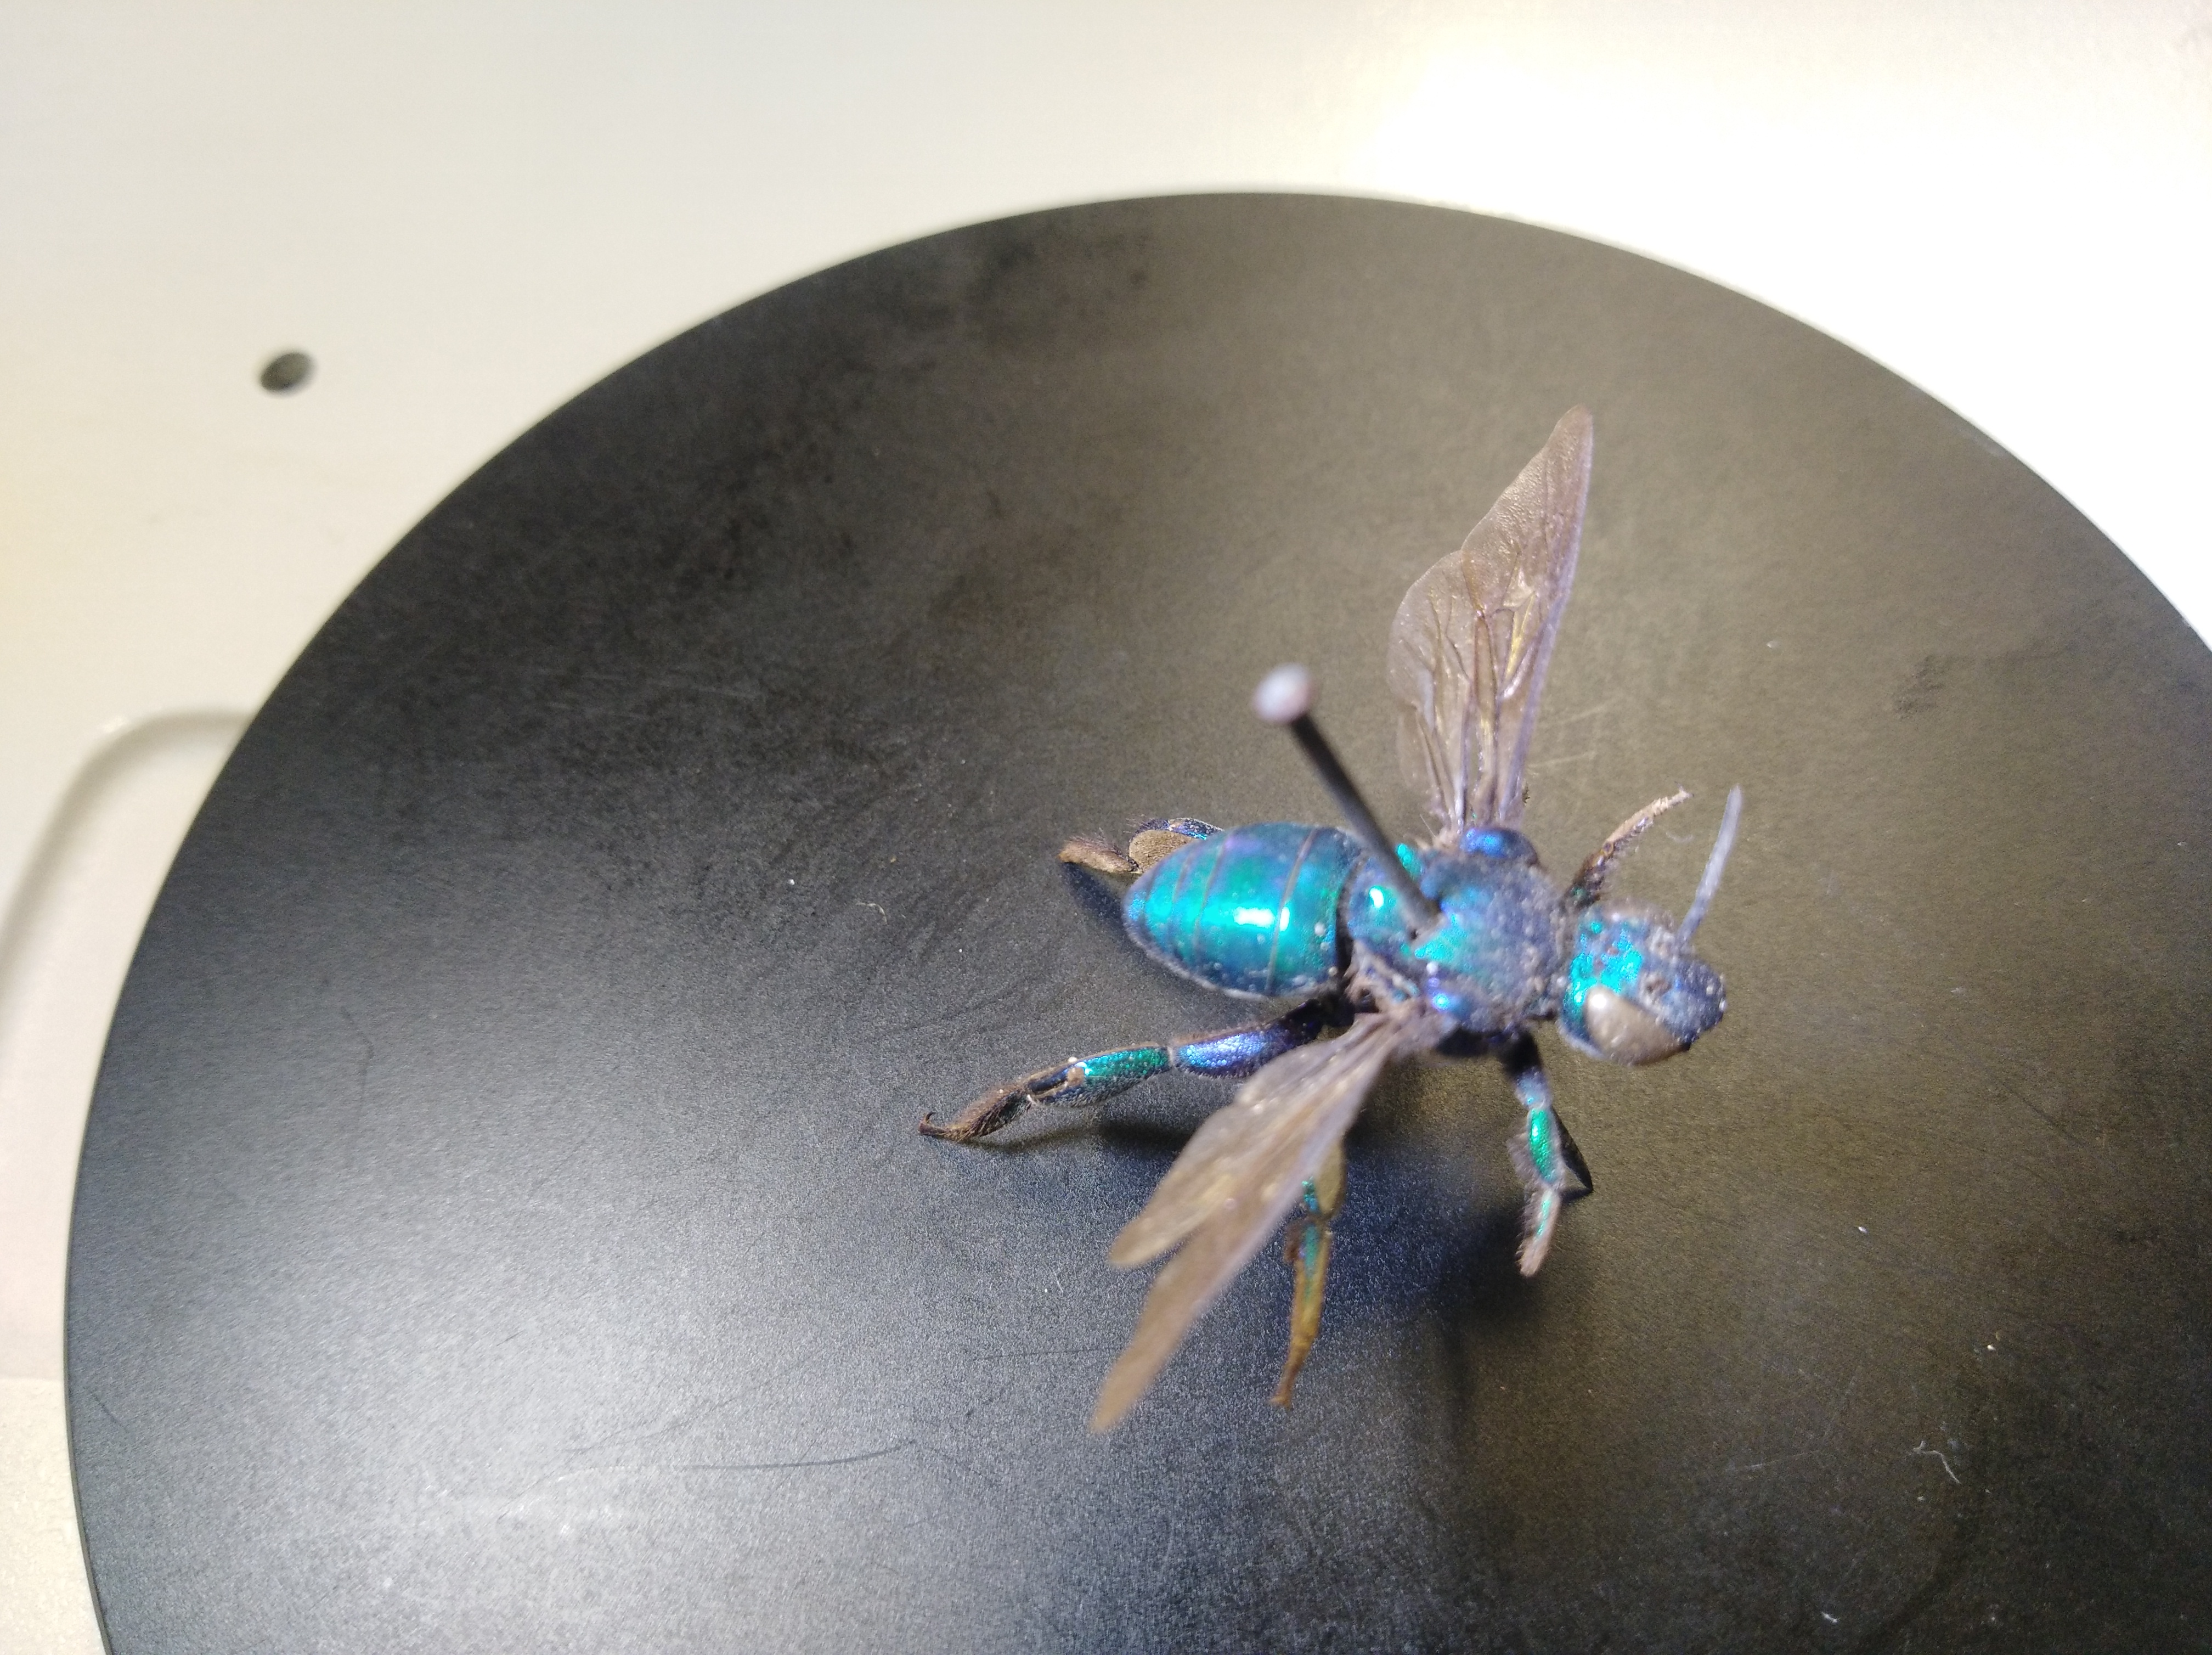
\includegraphics[width = 0.35\textwidth]{abeja.jpg}
    \caption{Abeja;Apidae}
    \label{tipos}
\end{figure}

\noindent Escarabajo de primero tipo:



\begin{figure}[H]
    \centering
    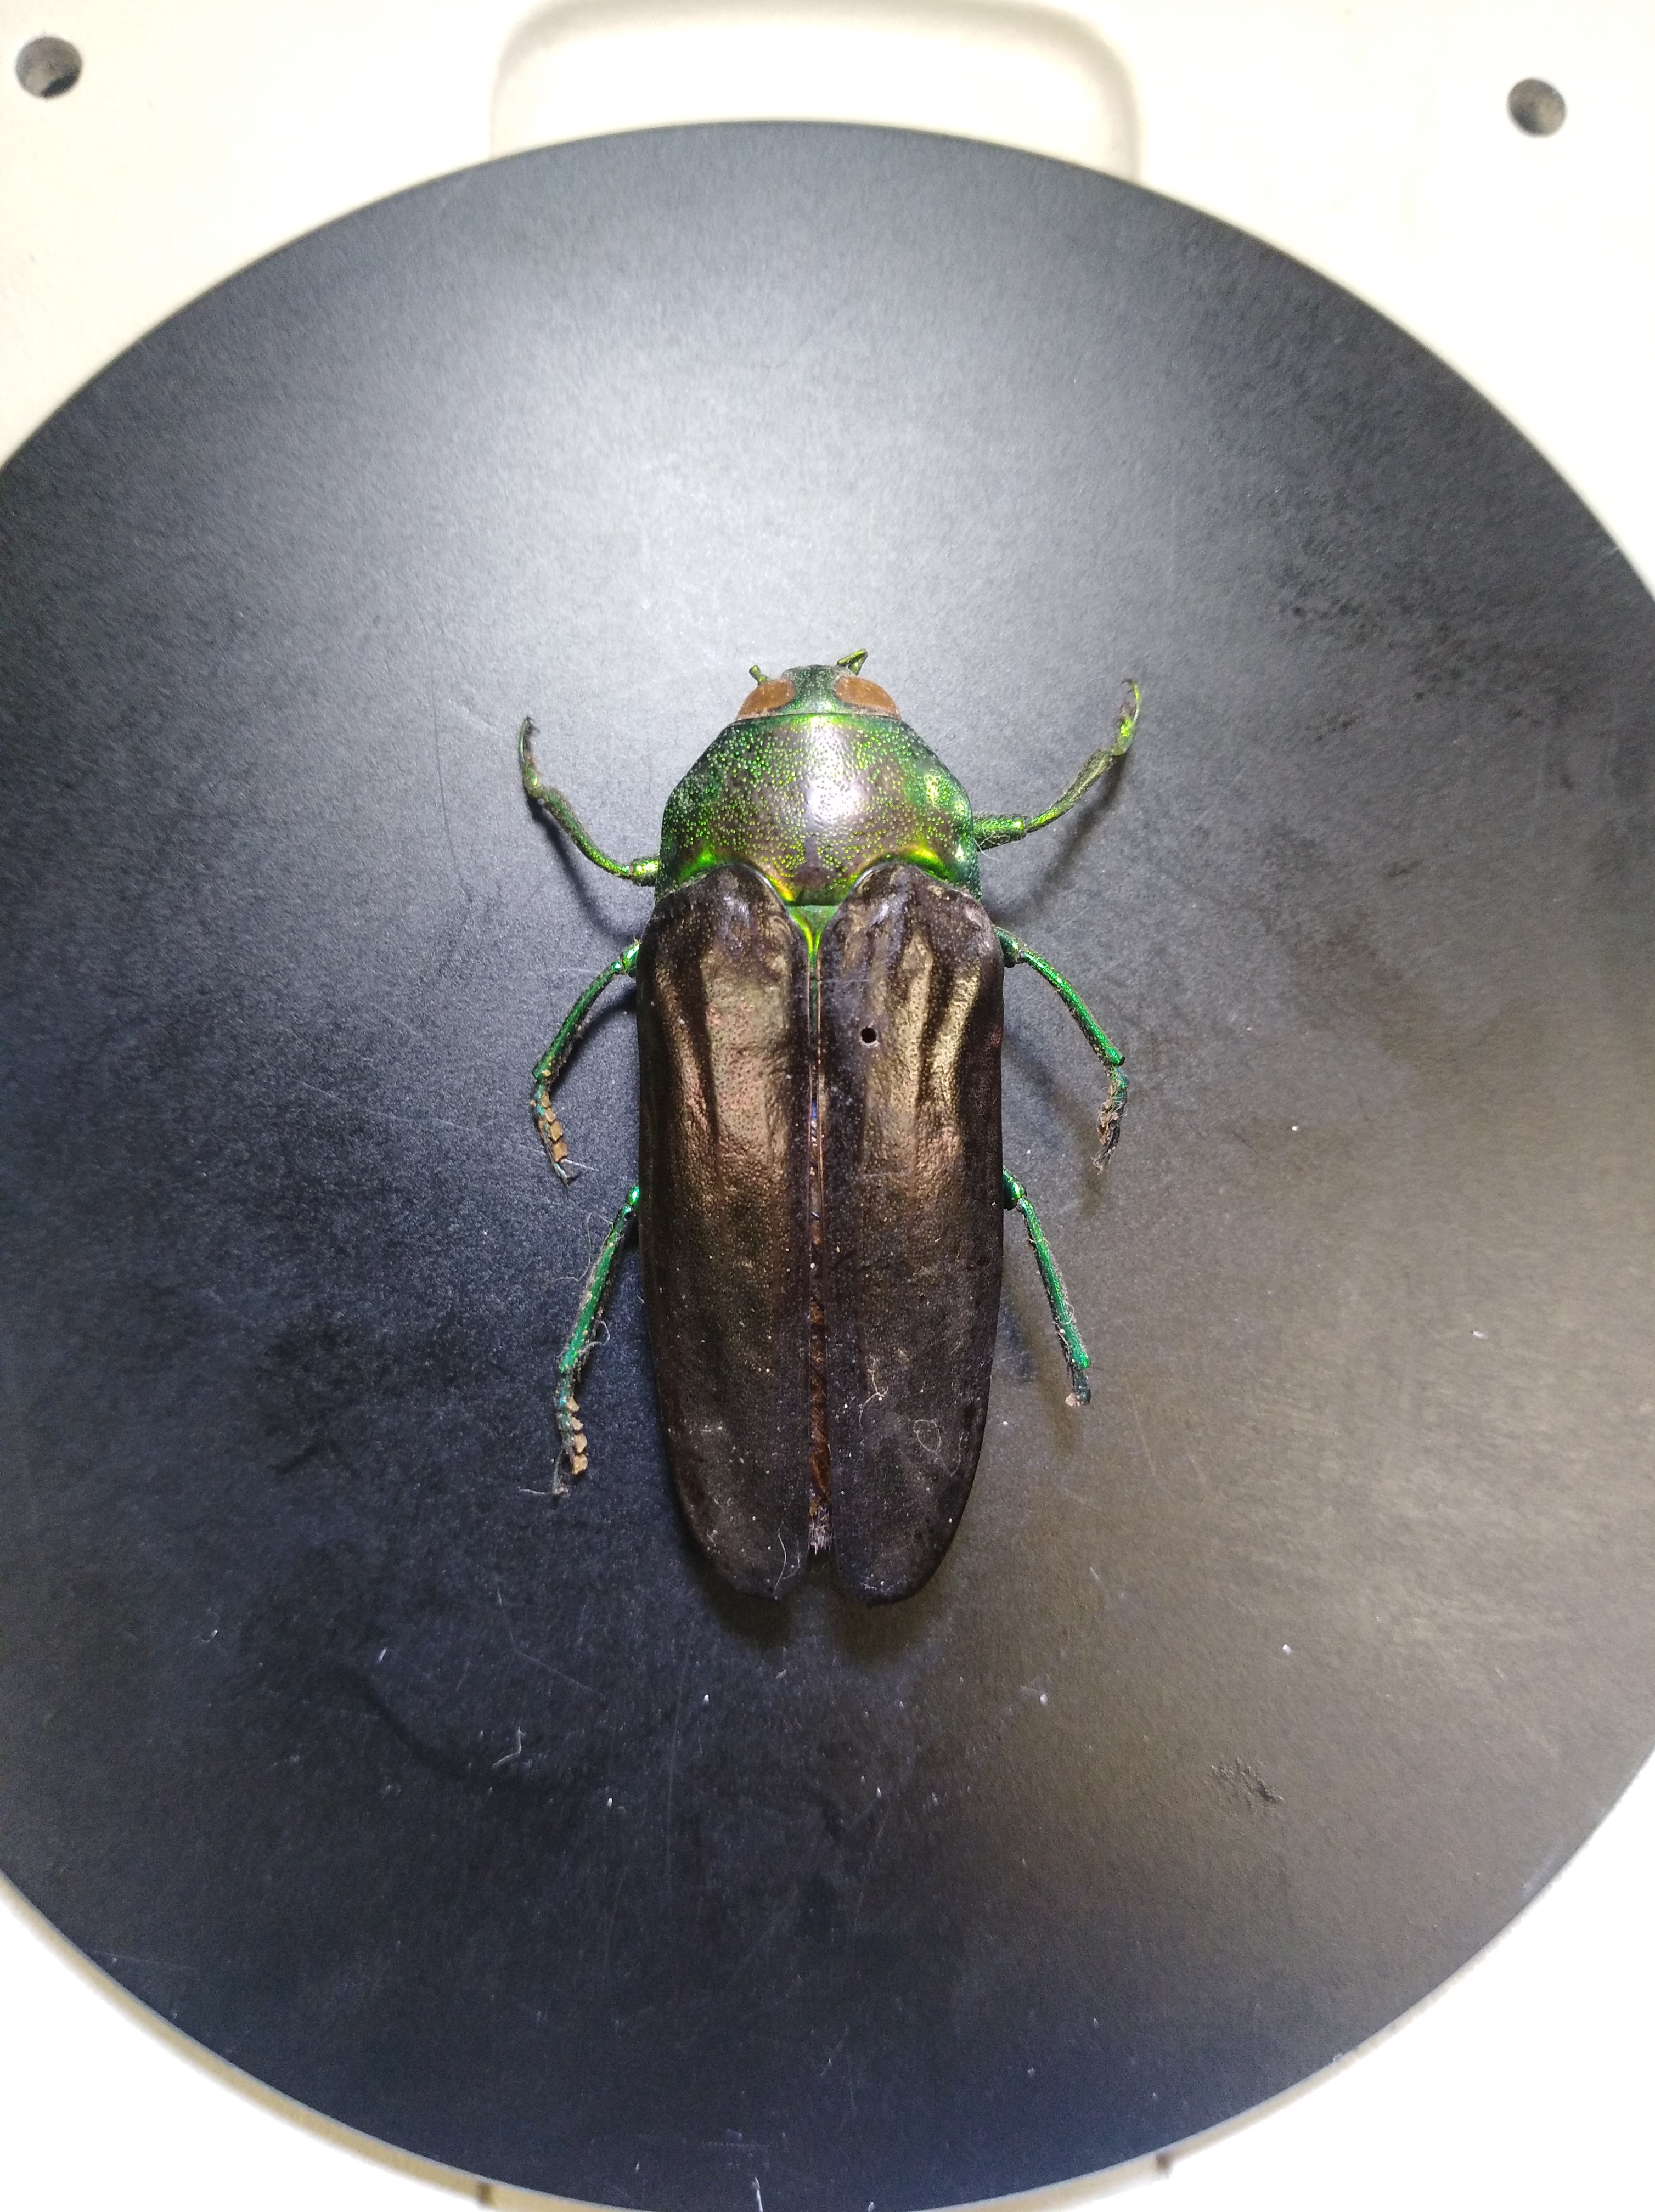
\includegraphics[width = 0.25\textwidth]{insecto1.jpg}
    \caption{insecto 1;Buprestidae tipo 1}
    \label{tipos}
\end{figure}

\noindent Escarabajo segundo tipo:


\begin{figure}[H]
    \centering
    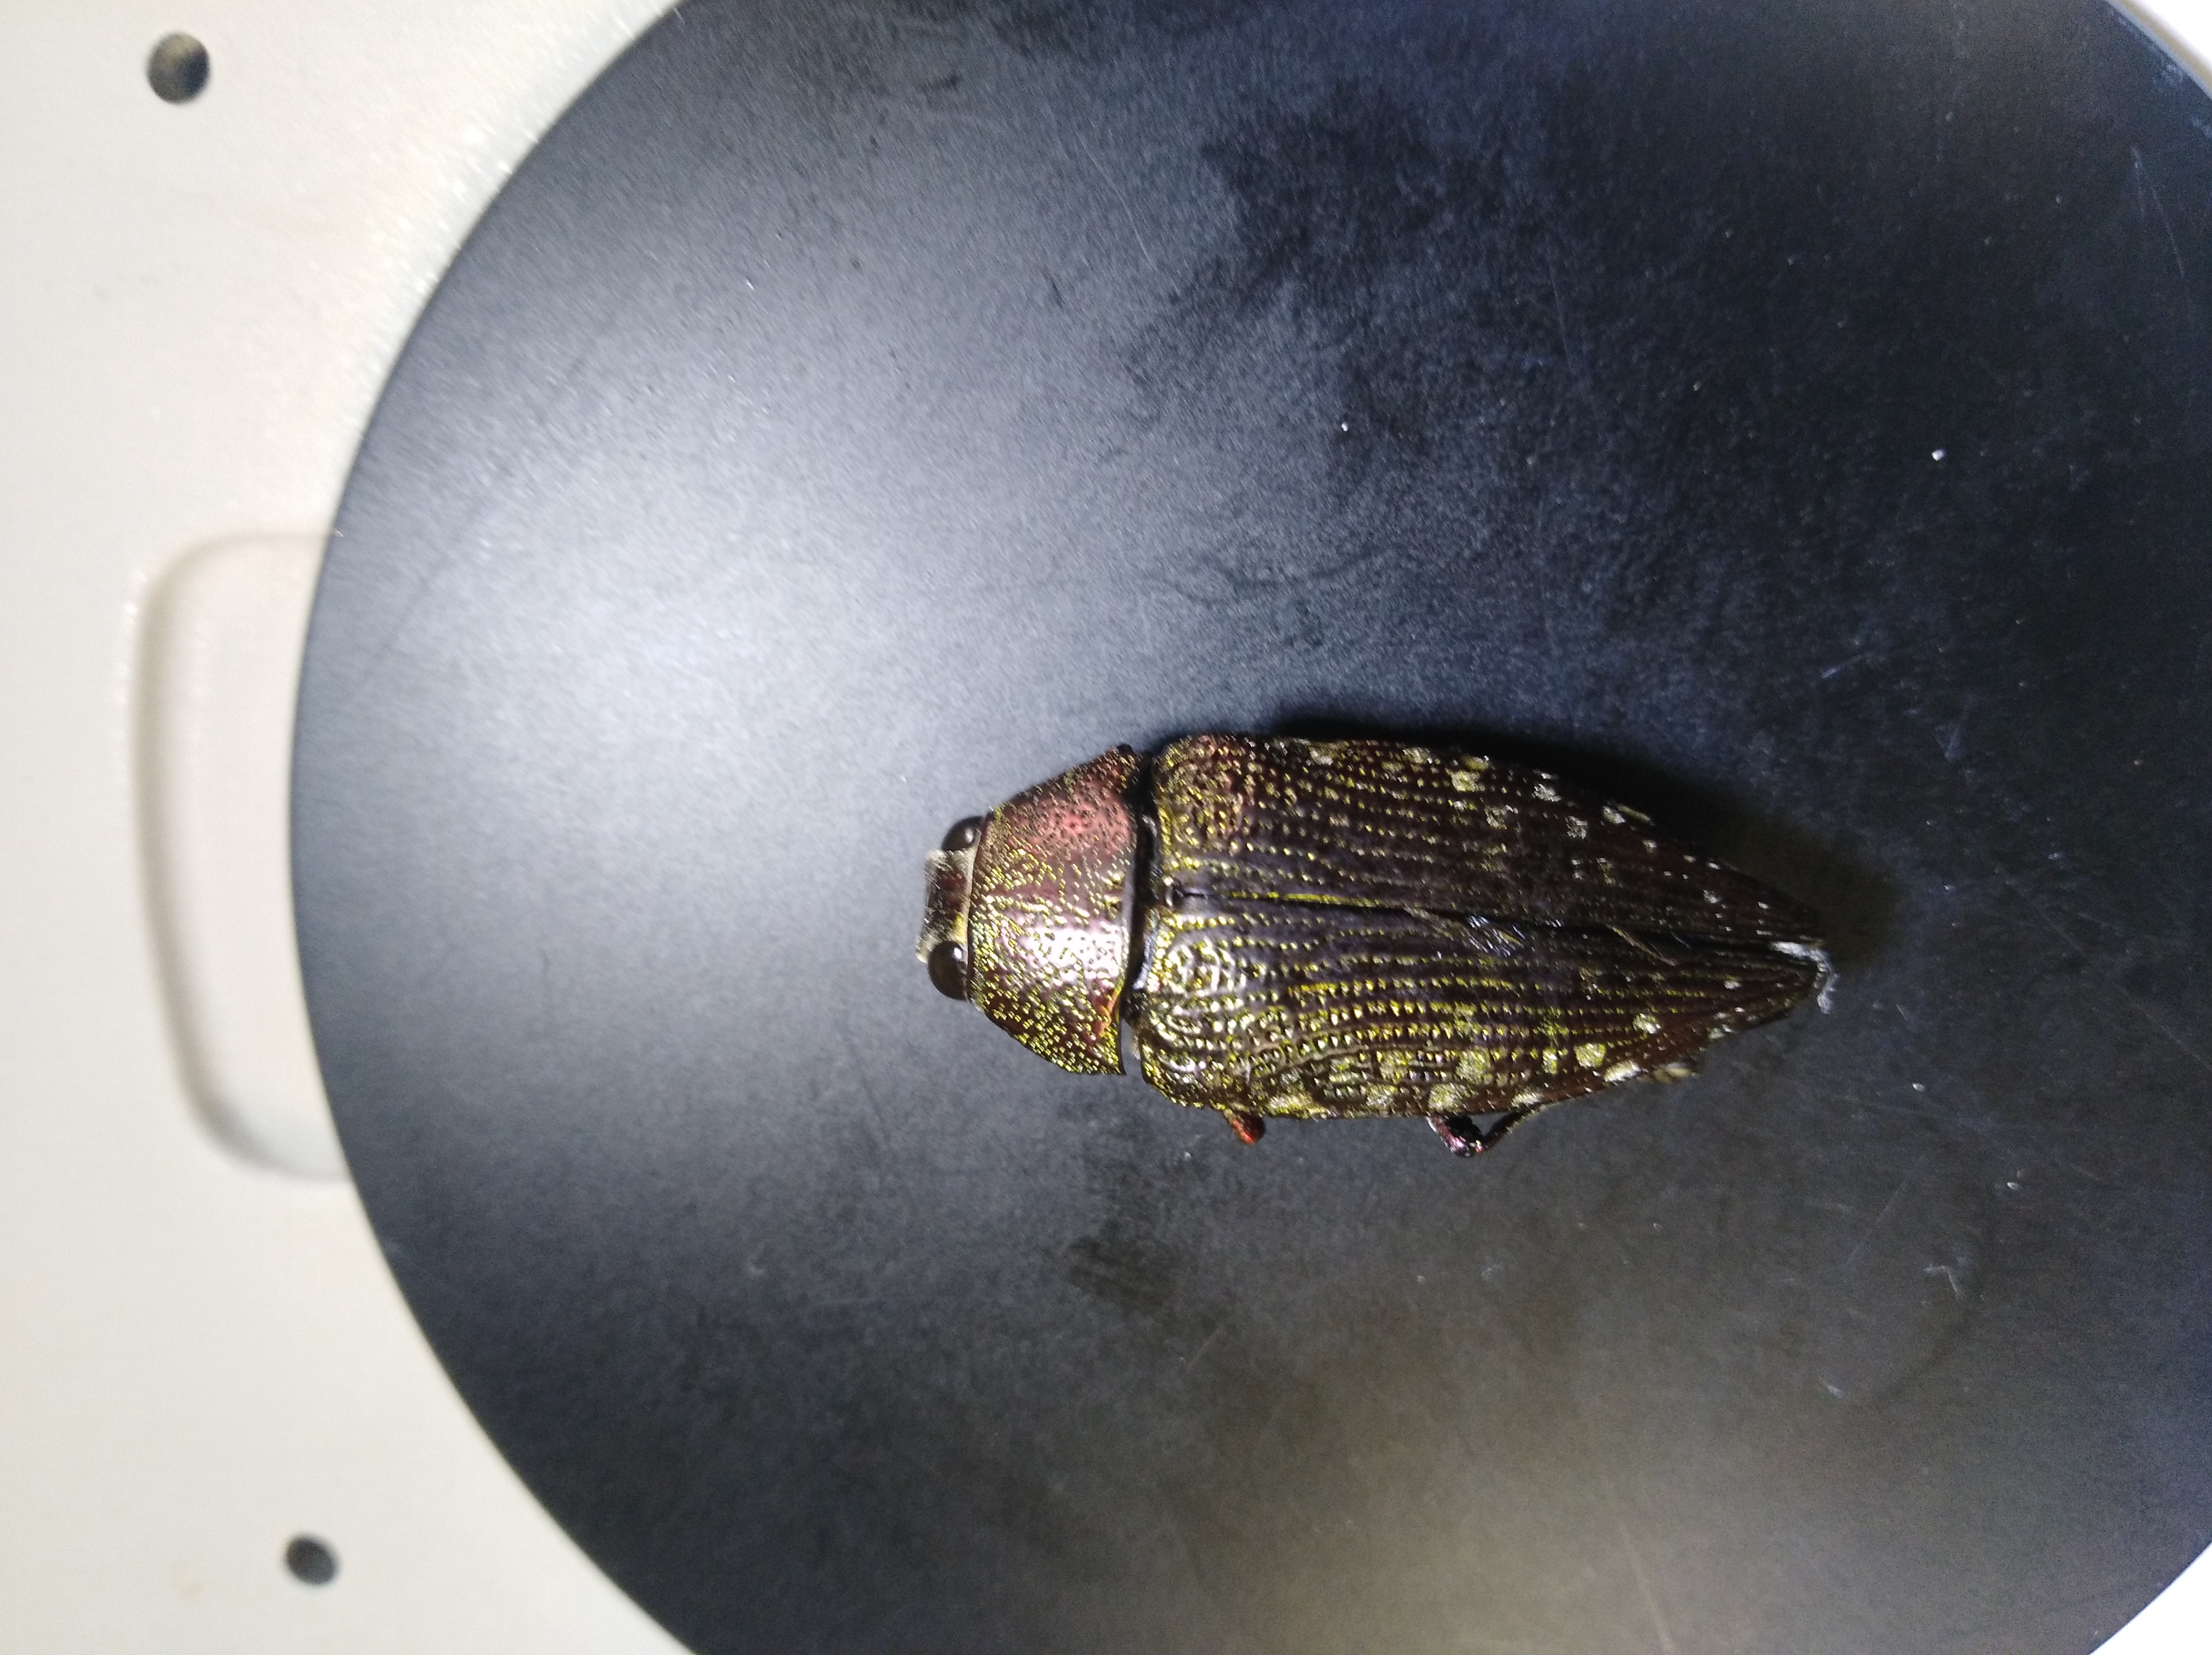
\includegraphics[width = 0.25\textwidth]{insecto2.jpg}
    \caption{Insecto 2;Buprestidae tipo 2}
    \label{tipos}
\end{figure}

\noindent Escarabajo de tercer tipo: 

\begin{figure}[H]
    \centering
    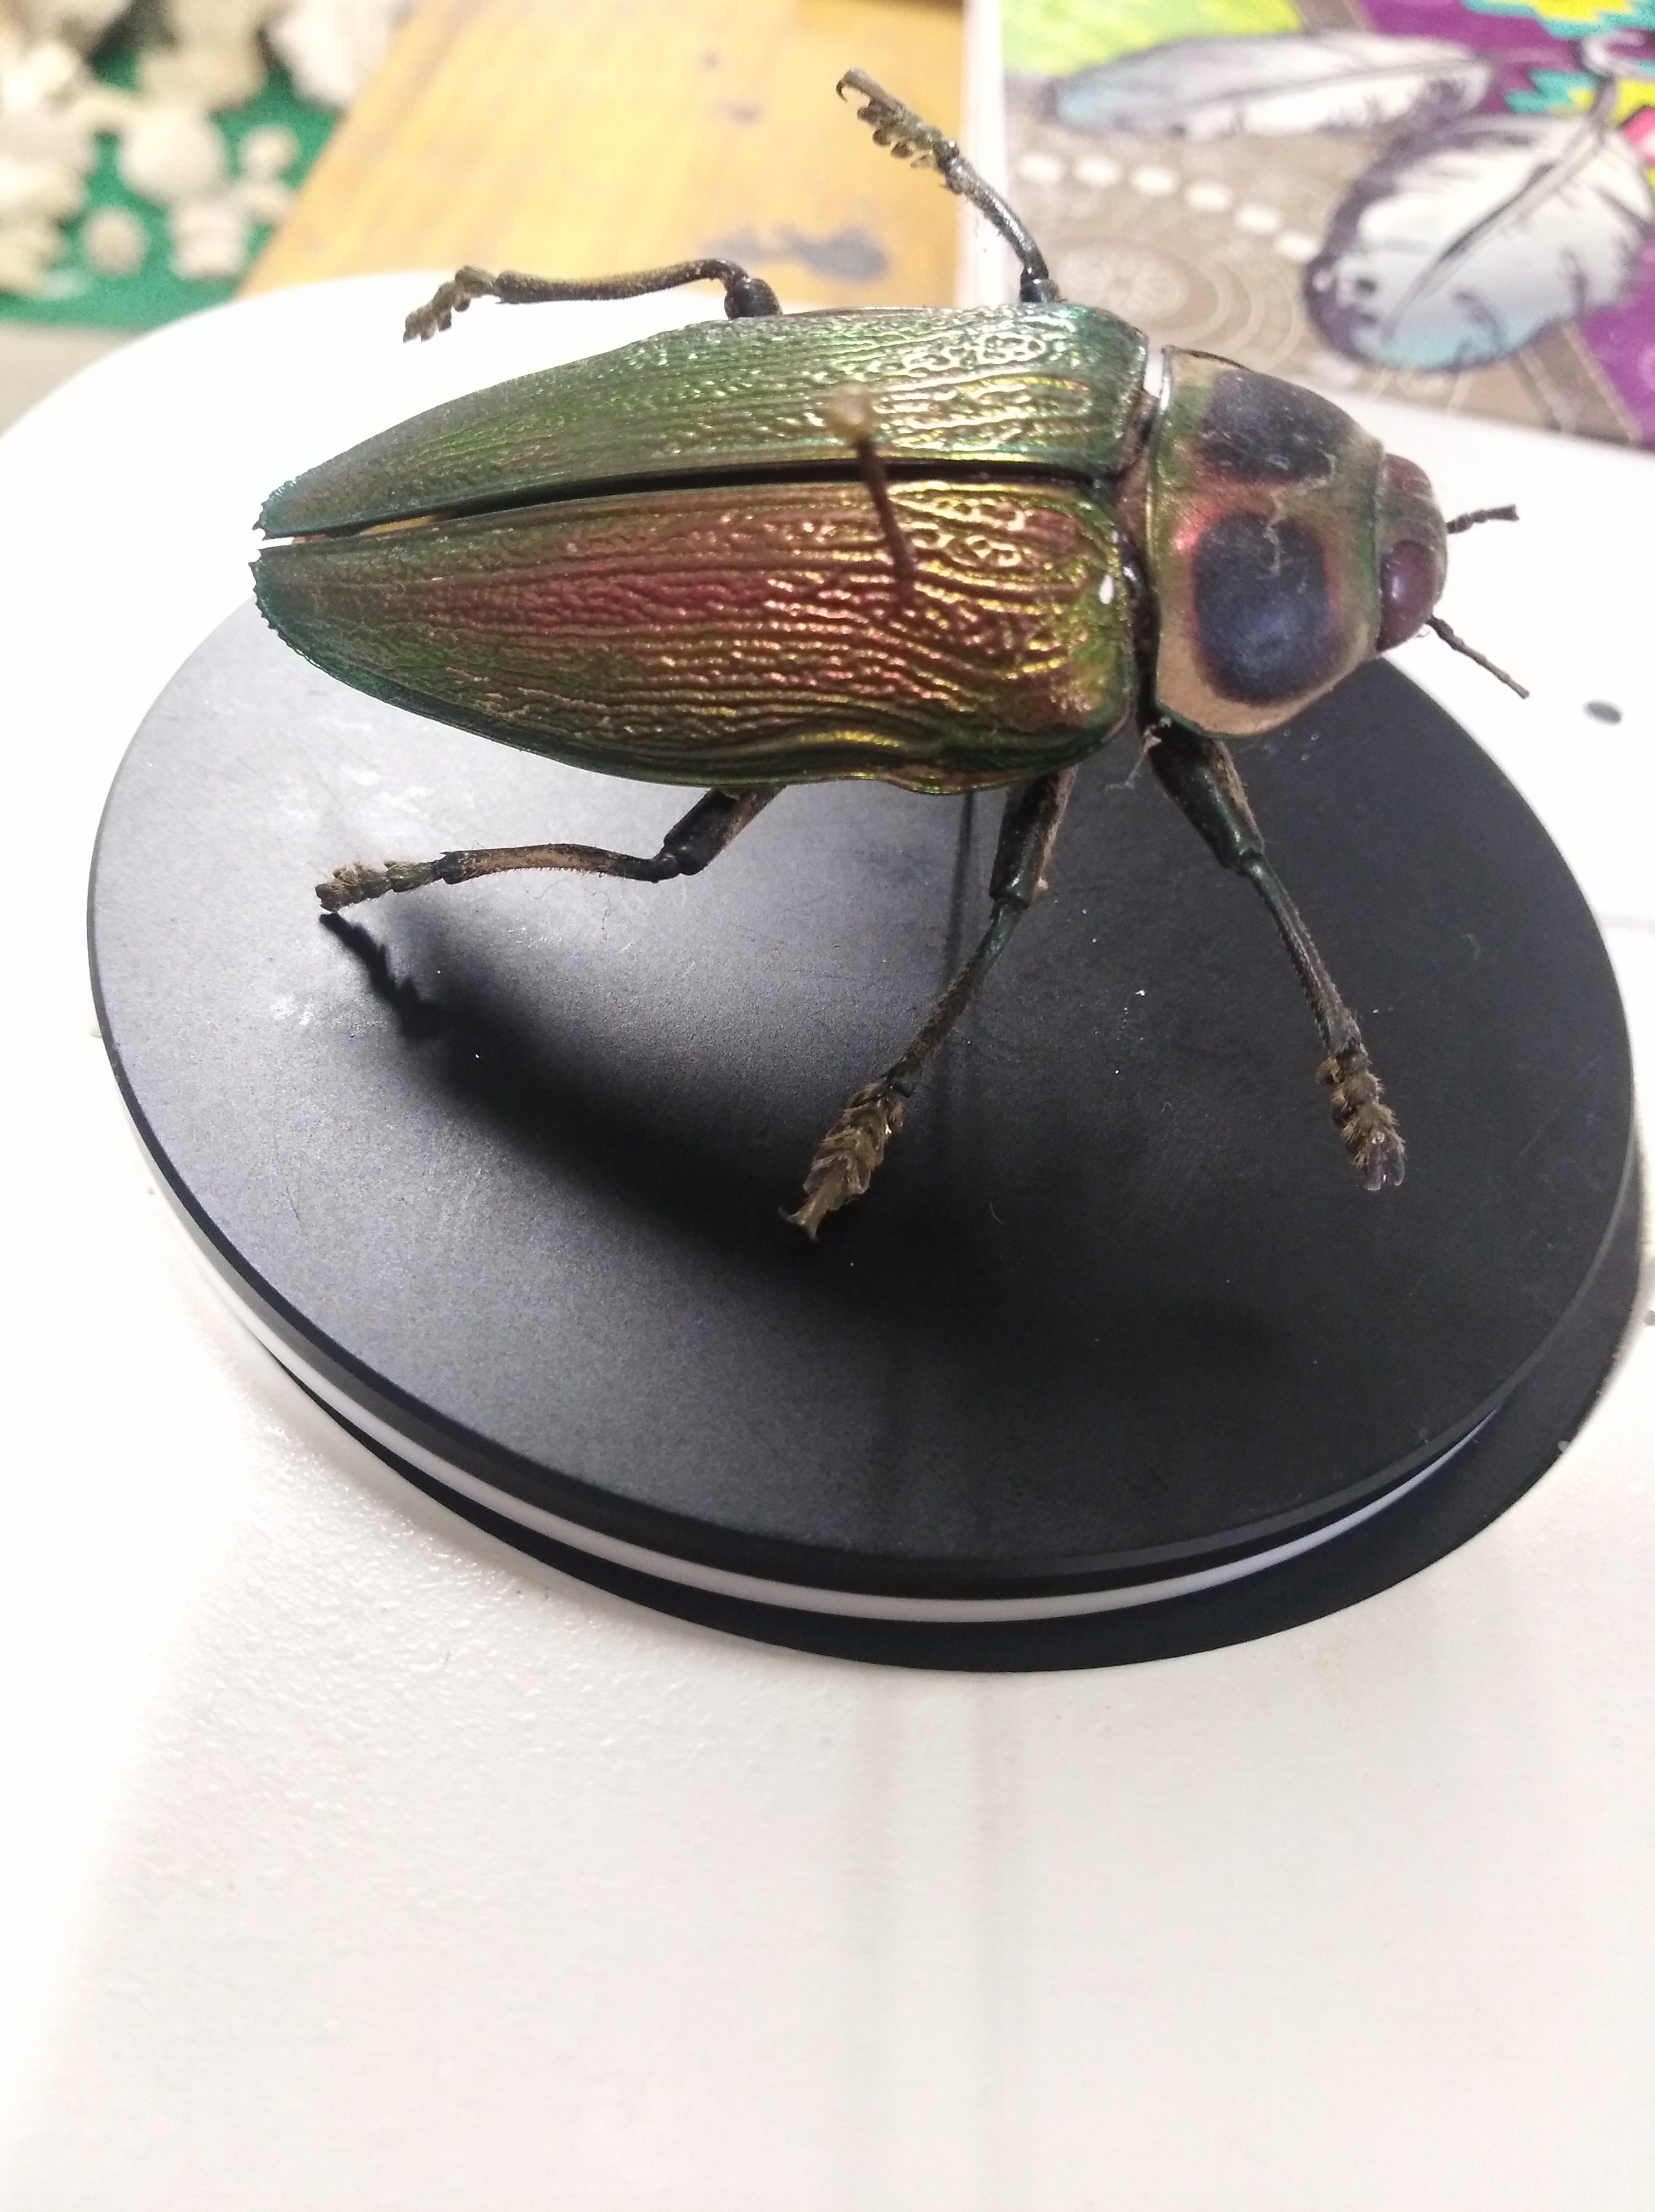
\includegraphics[width = 0.25\textwidth]{insecto3.jpg}
    \caption{Insecto 3; Scarabaeidae}
    \label{tipos}
\end{figure}

\noindent Cigarra estándar


\begin{figure}[H]
    \centering
    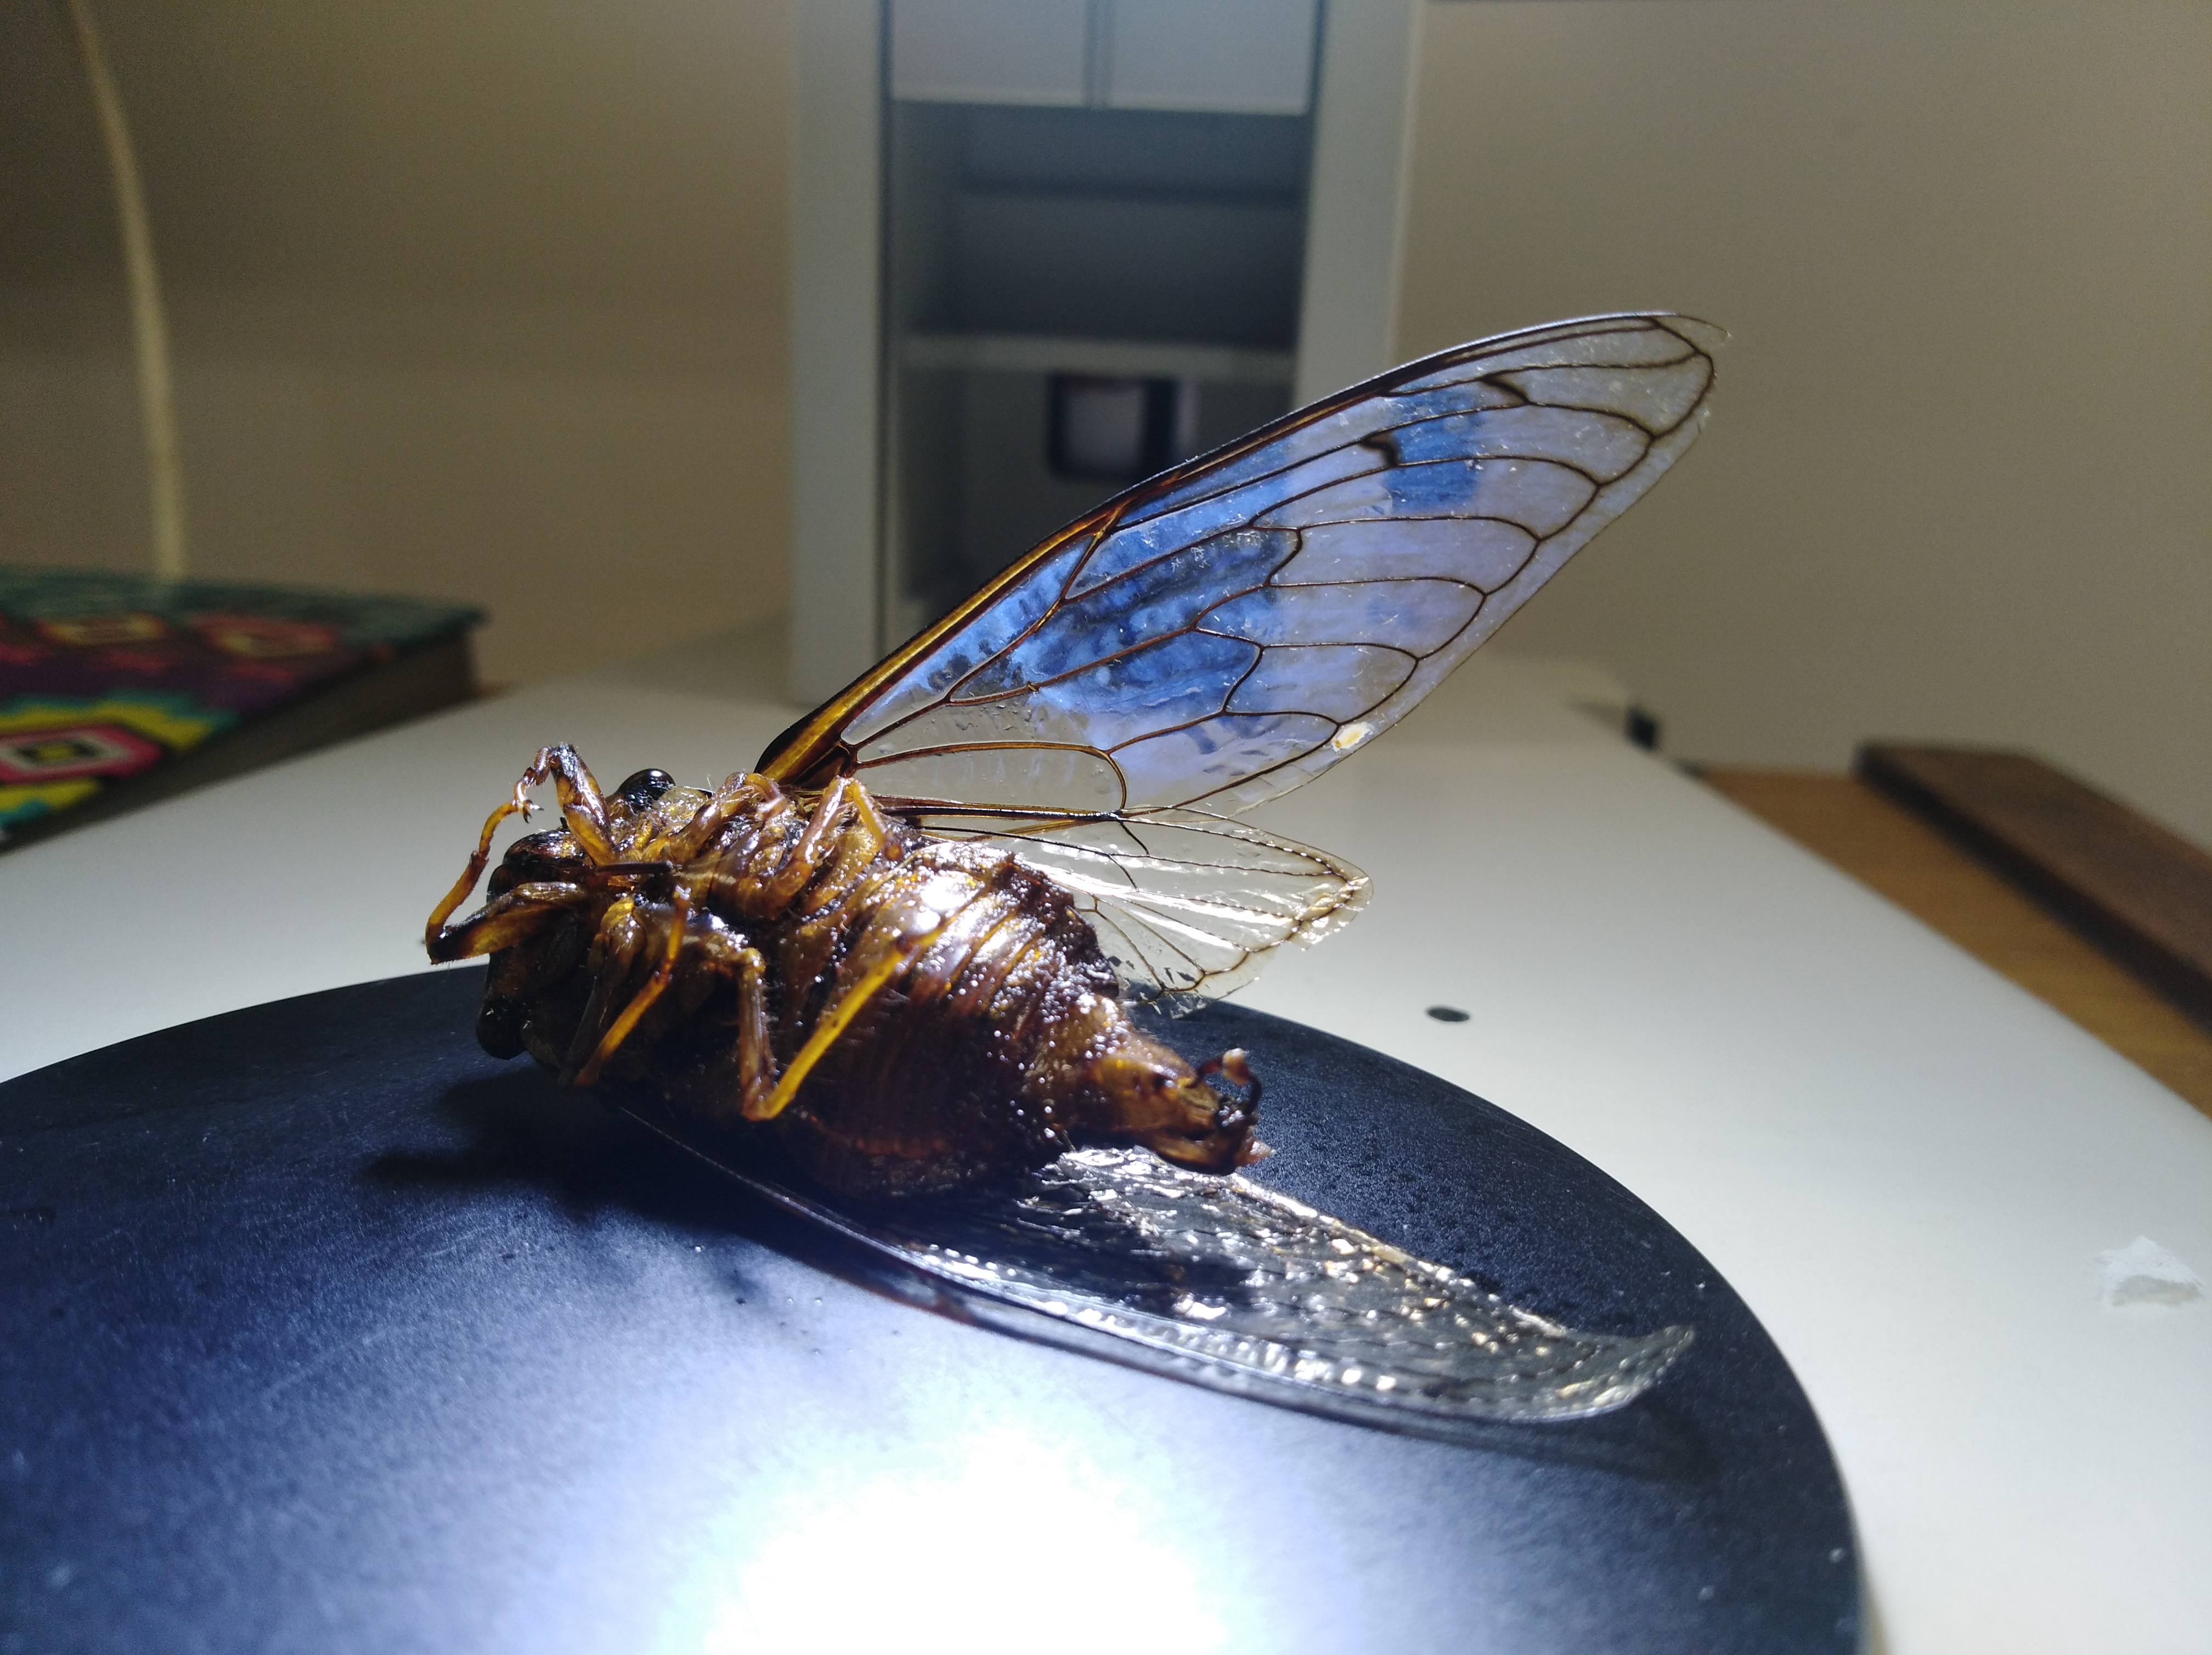
\includegraphics[width = 0.25\textwidth]{cigarra.jpg}
    \caption{Imagen de Cigarra}
    \label{tipos}
\end{figure}

\noindent Para la segunda fase se pusieron sobre un microscópio estereoscópico para observar más de cerca la estructura sobre sus caparazones o alas con el fin de obtener un acercamiento a la microestructura presente en cada insecto.

El microscópio implementado (20x) se muestra a continuación:

%fotoooo


\begin{figure}[H]
    \centering
    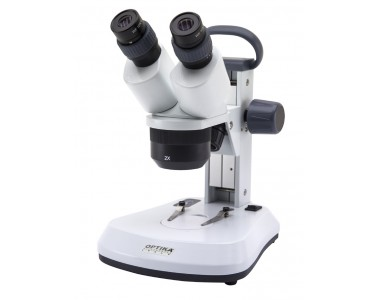
\includegraphics[width = 0.3\textwidth]{estereo.jpg}
    \caption{Microscópio estereoscópico implementado para realizar el respectivo acercamiento de la superficie de los insectoas y así poder observar su microestructura}
    \label{tipos}
\end{figure}



\section*{Resultados}

Una vez puestos cada insecto en el microscópio, se hallaron las siguientes estructuras:

\noindent Para la abeja; Apidae:

\begin{figure}[H]
    \centering
    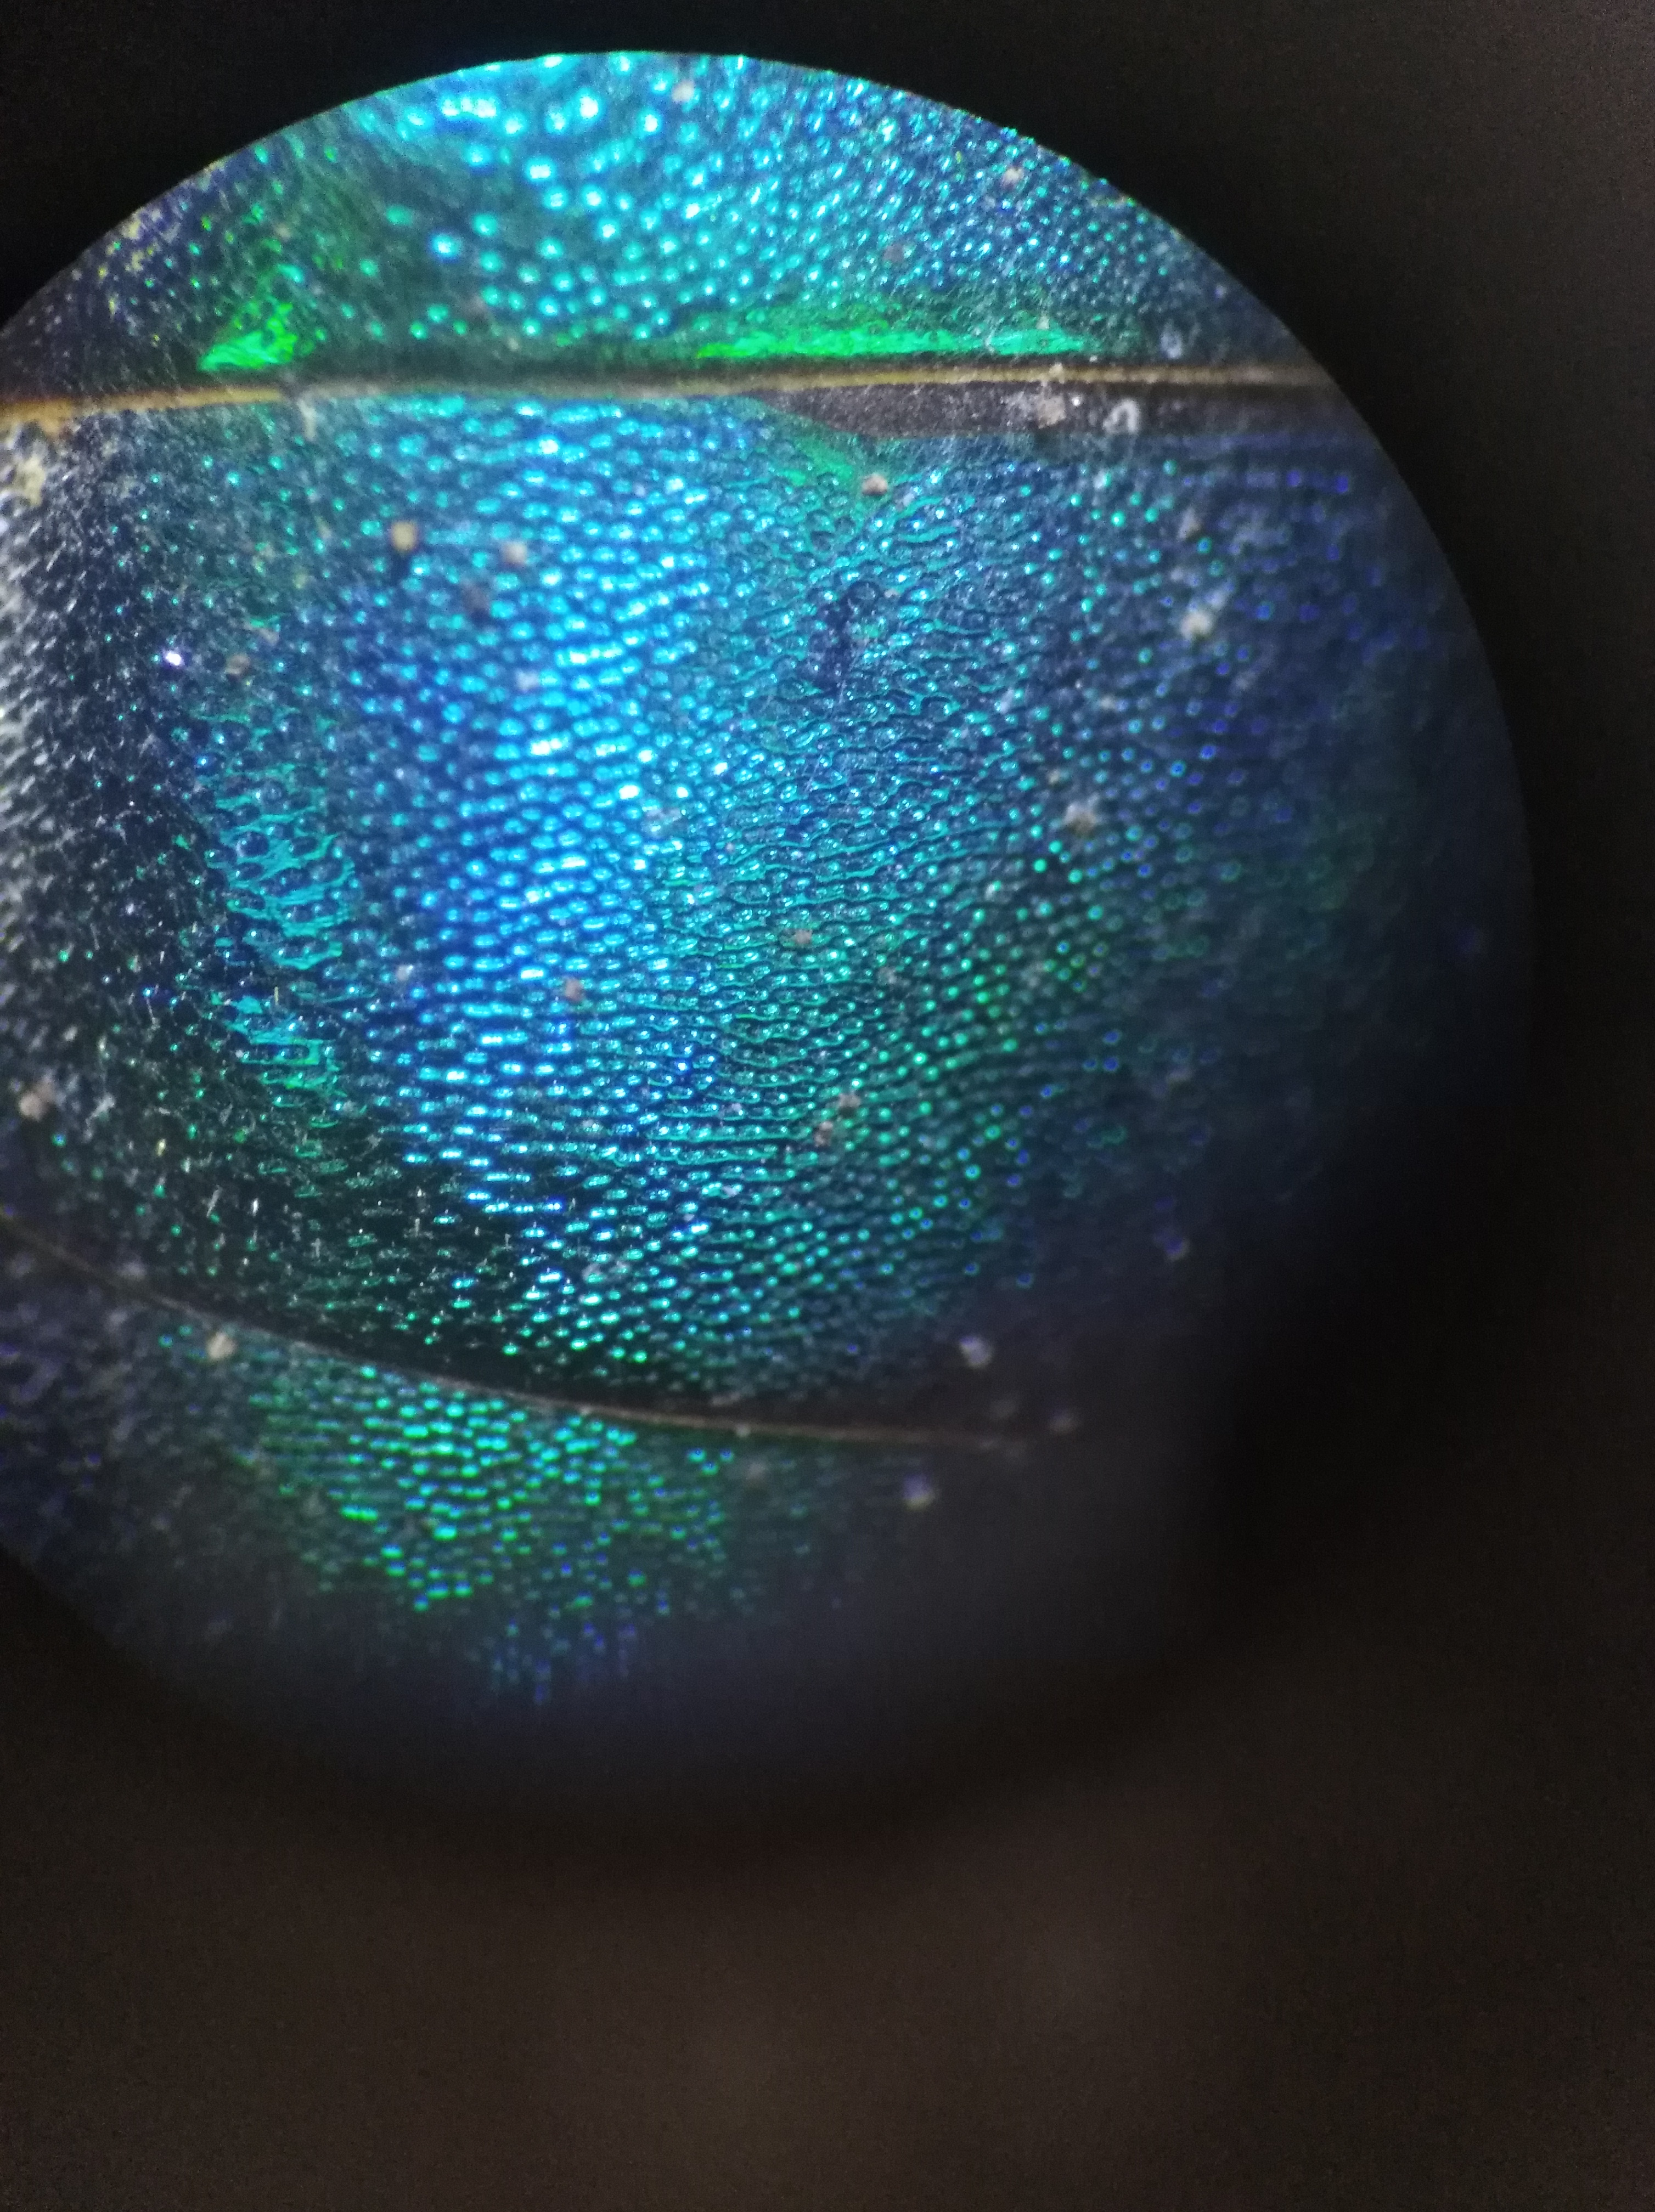
\includegraphics[width = 0.25\textwidth]{puntos_abeja.jpg}
    \caption{Superficie de la Apidae}
    \label{tipos}
\end{figure}

\noindent Primer escarabajo: Buprestidae tipo 1:

\begin{figure}[H]
    \centering
    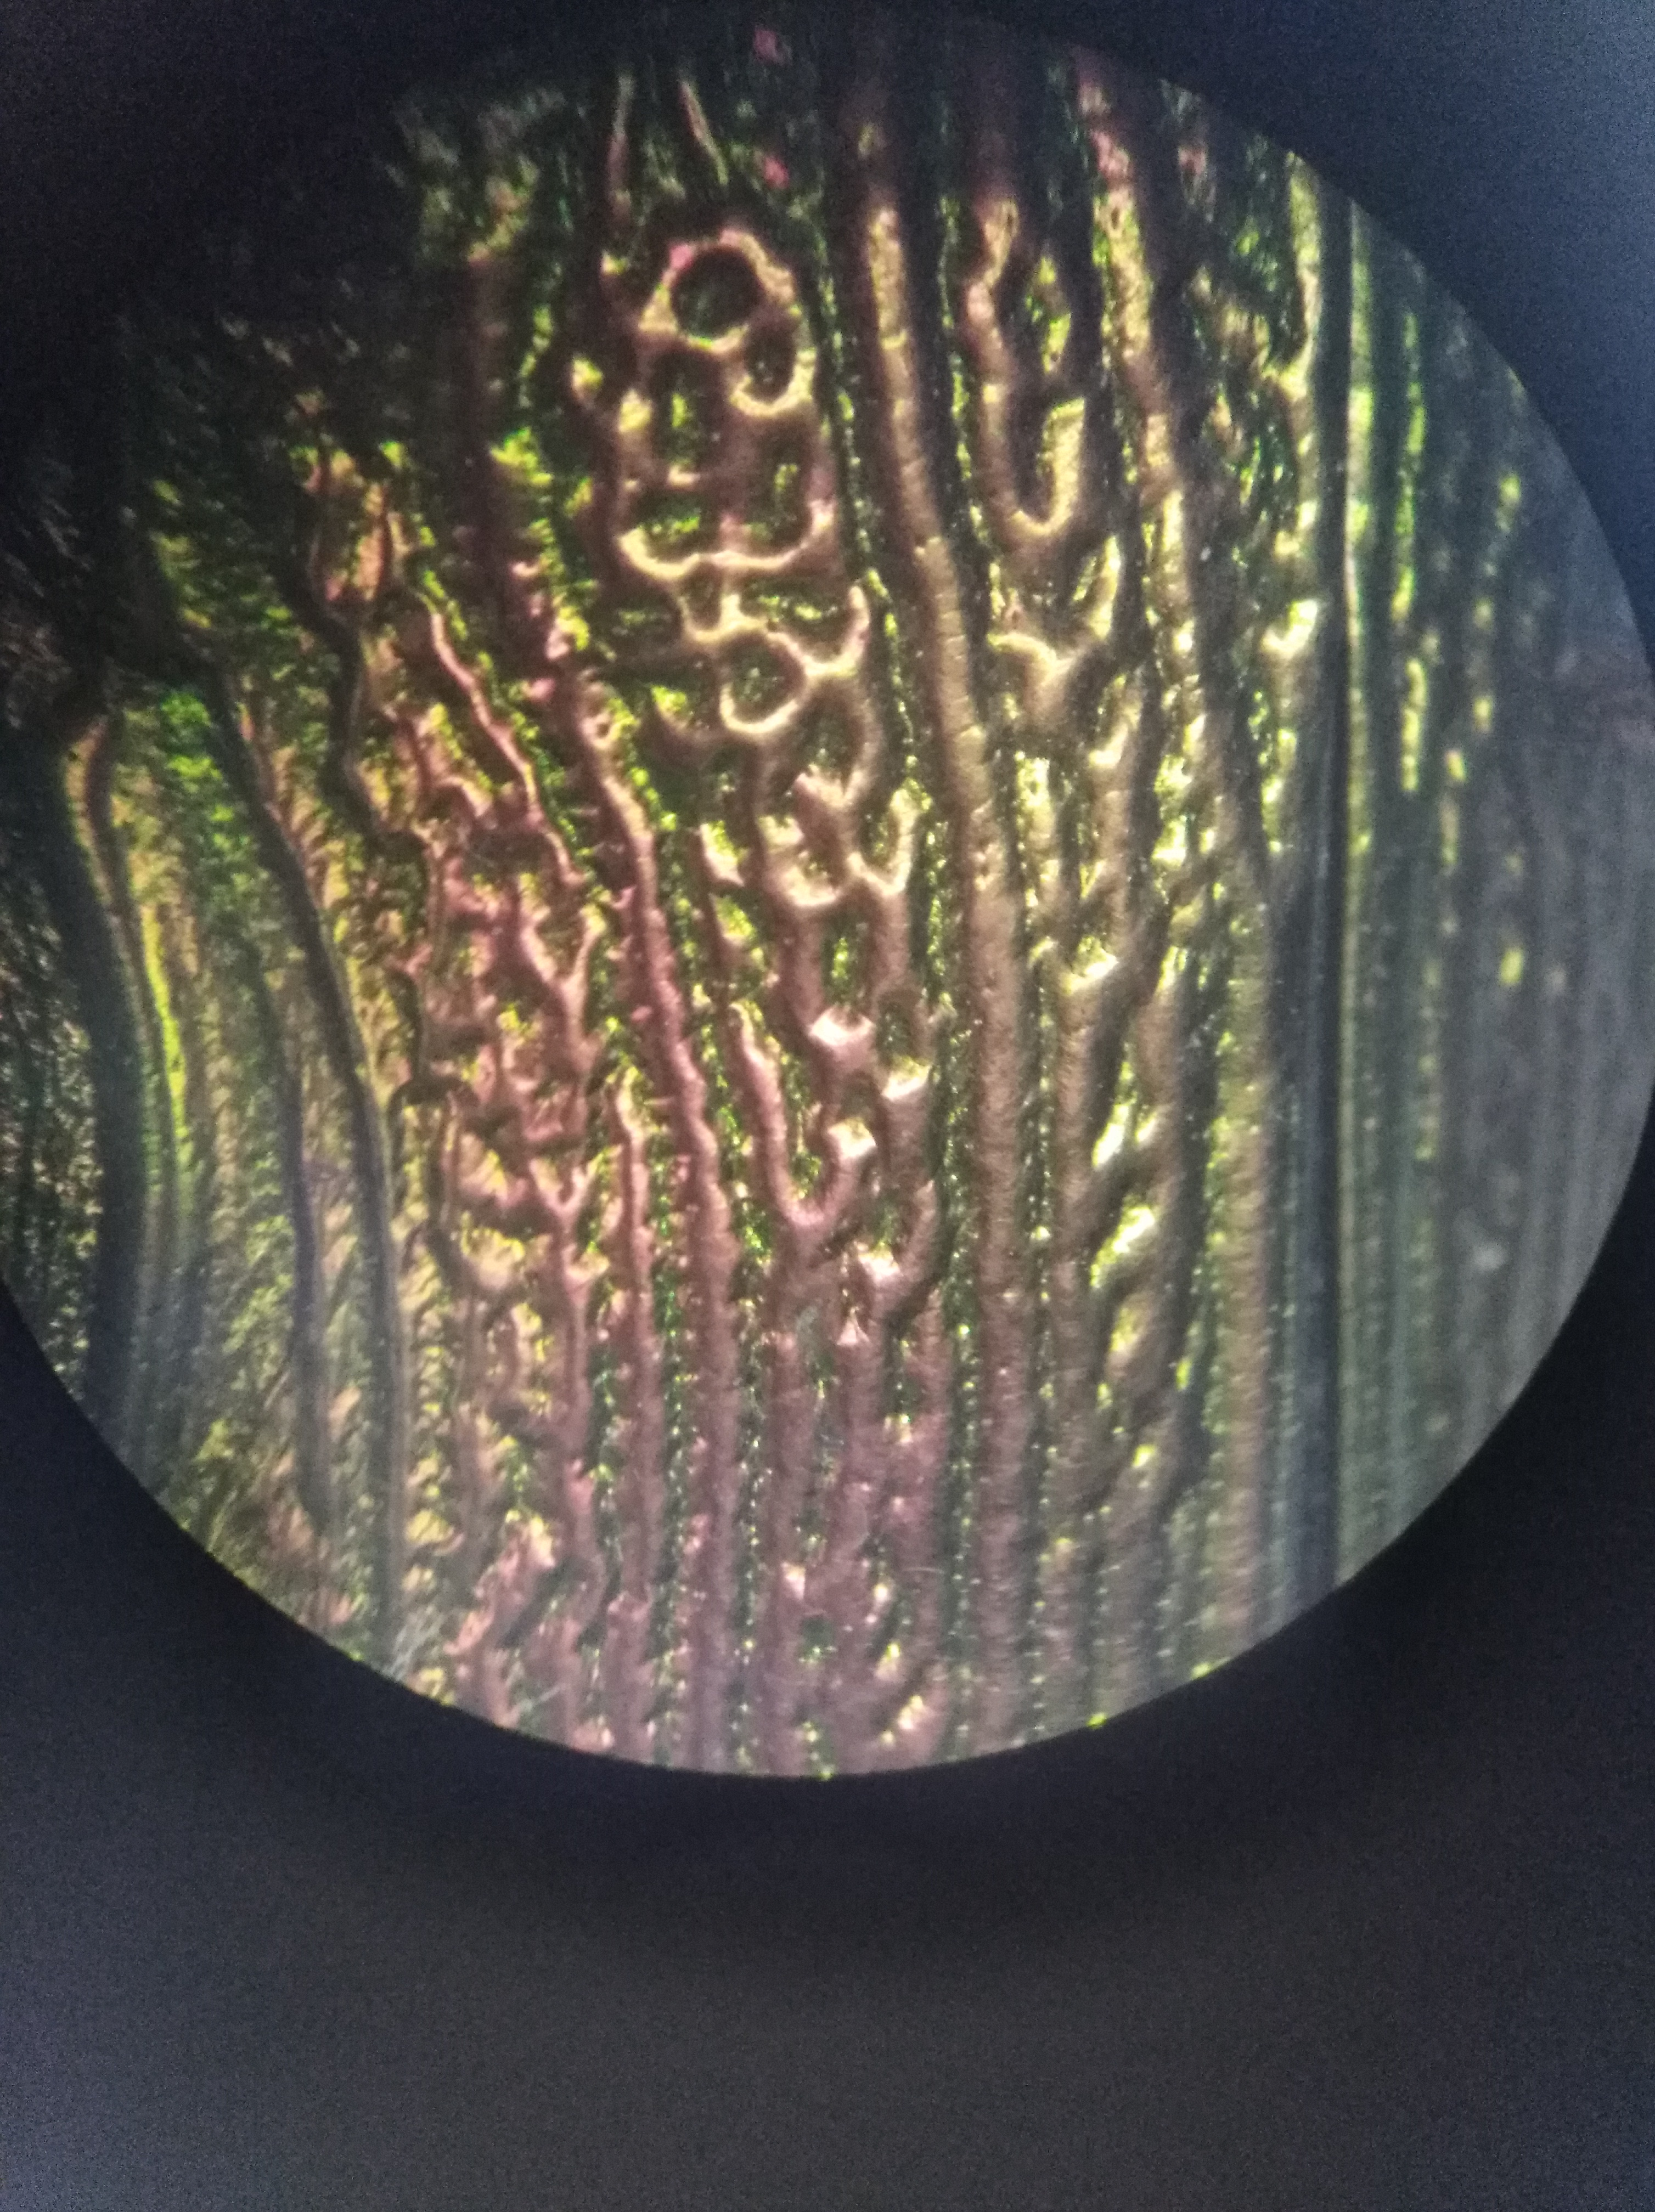
\includegraphics[width = 0.25\textwidth]{insecto1_arriba.jpg}
    \caption{Parte Dorsal del Buprestidae tipo 1}
    \label{fig:DorsalB1}
\end{figure}


\begin{figure}[H]
    \centering
    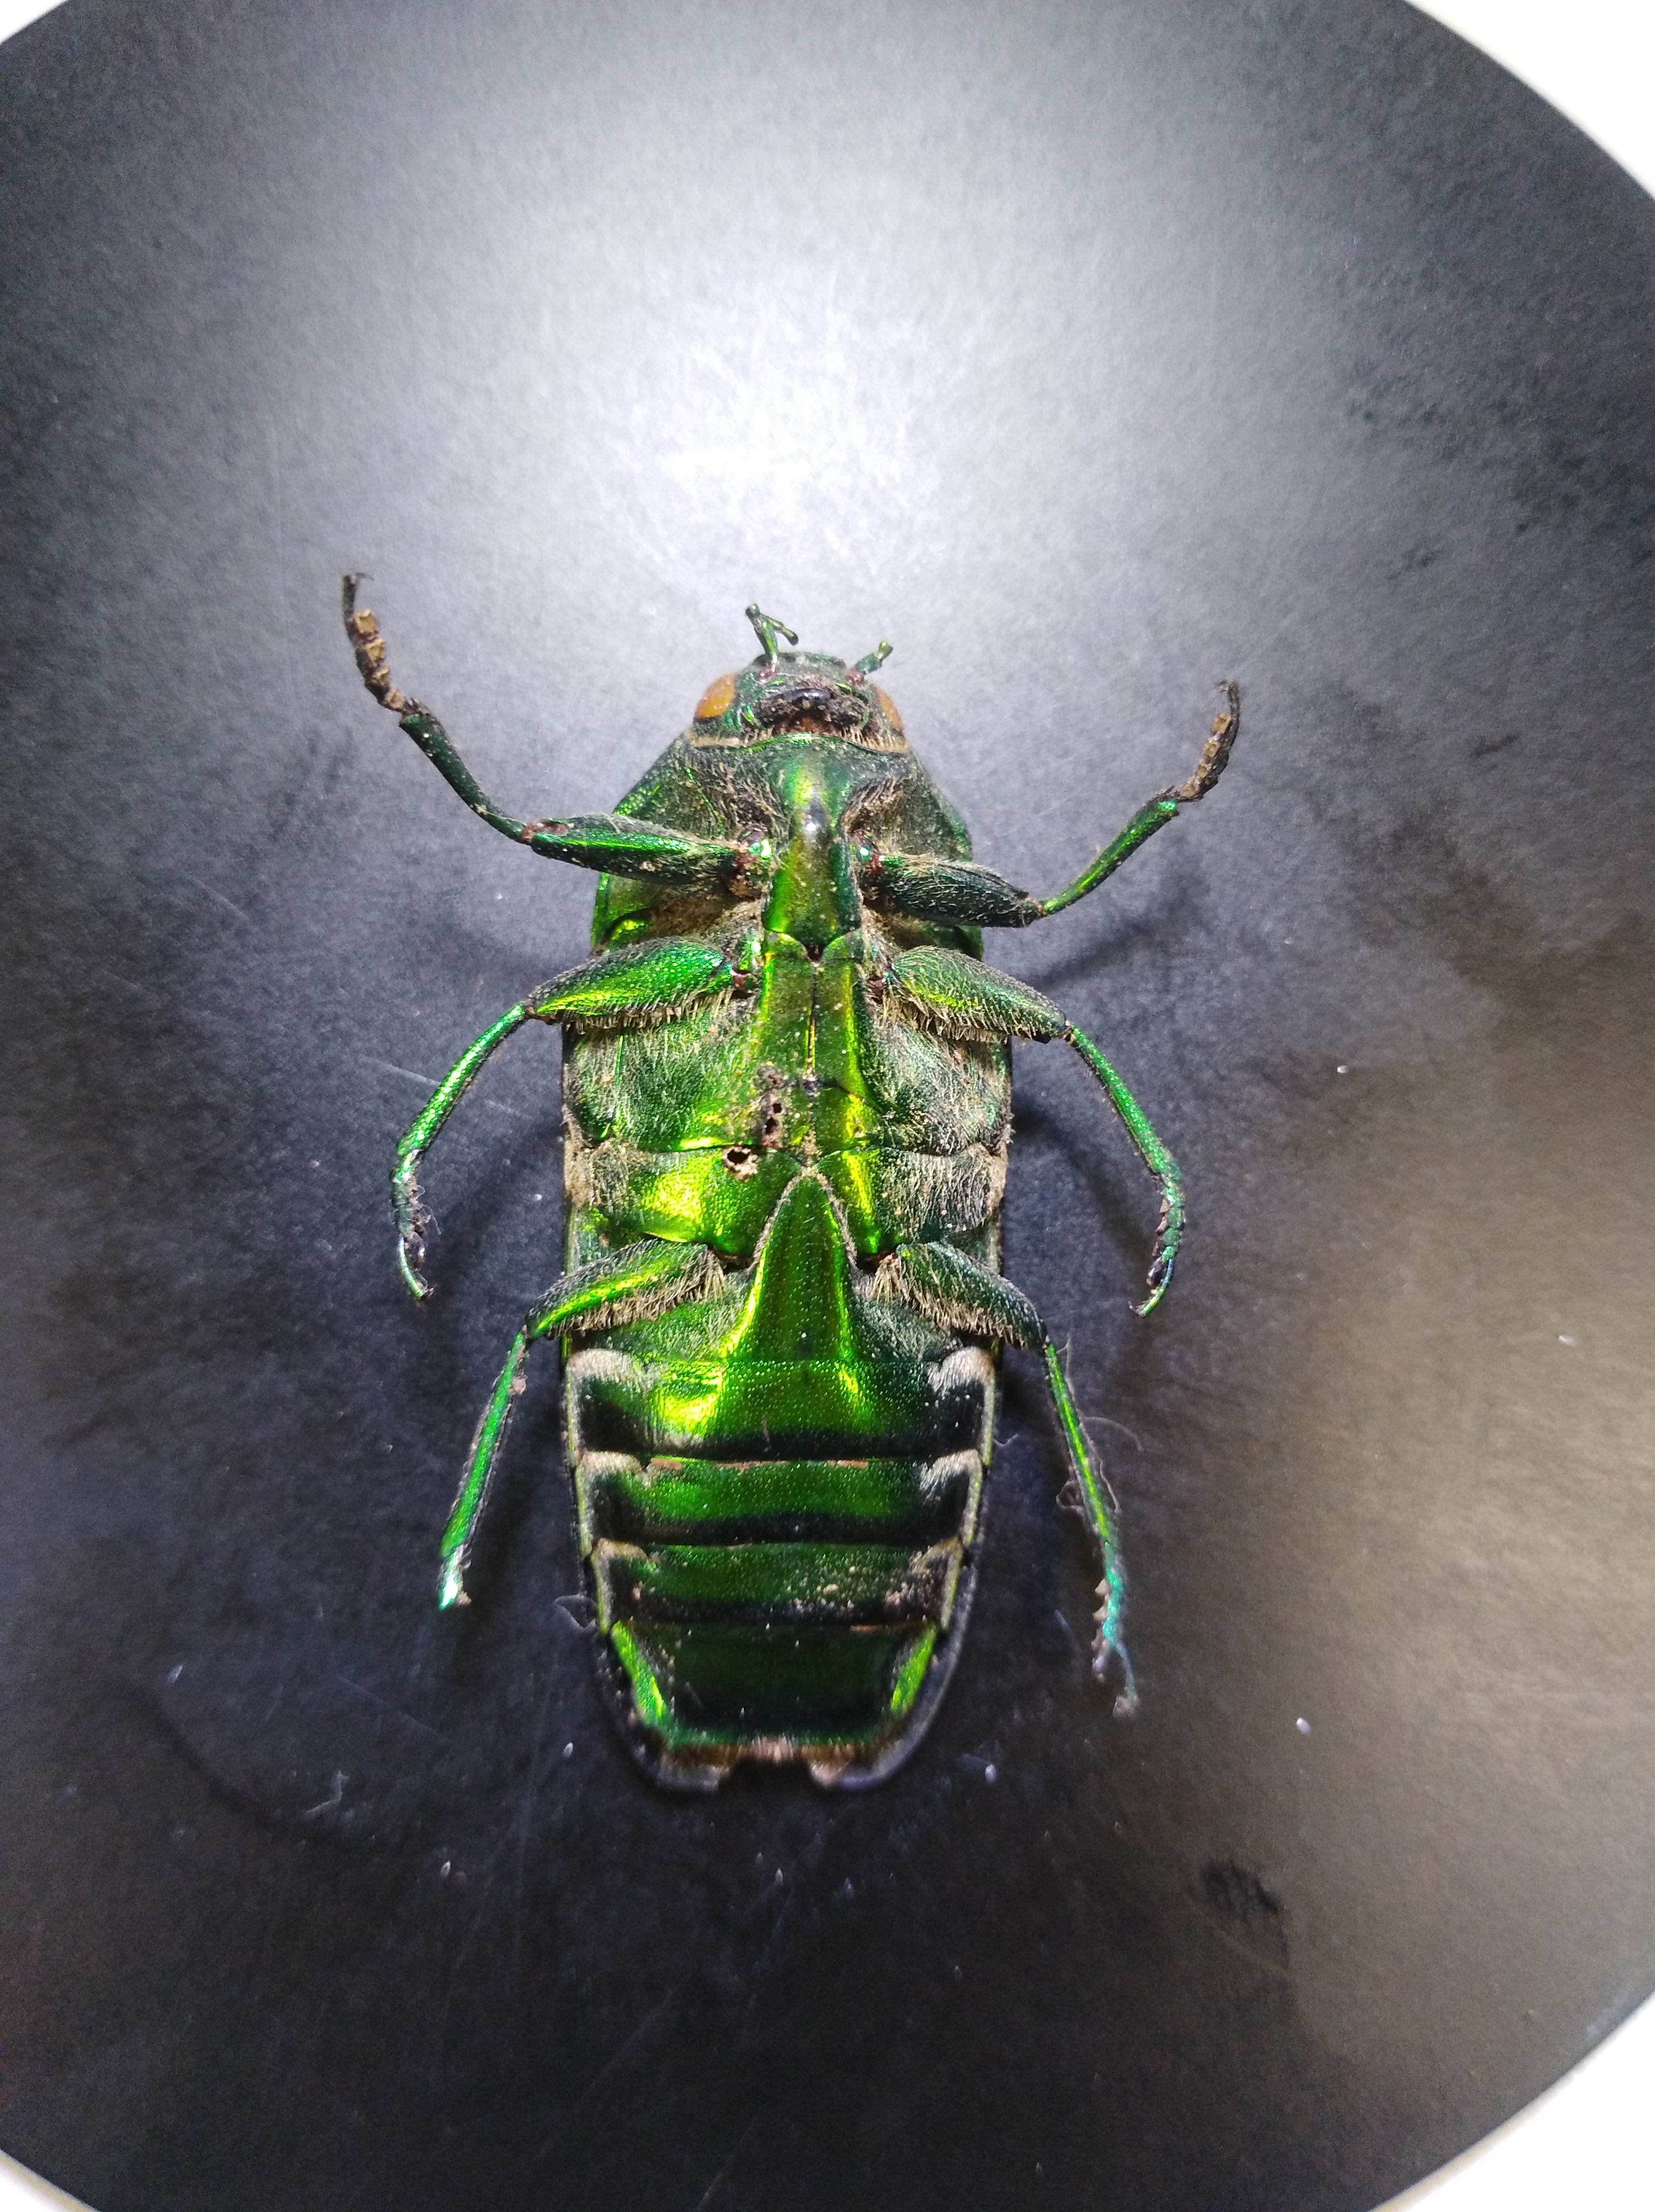
\includegraphics[width=0.25\textwidth]{insecto1_abajo_todo.jpg}
    \caption{Parte Ventral del Buprestidae tipo 1}
    \label{fig:VentralB1}
\end{figure}

\begin{figure}[H]
    \centering
    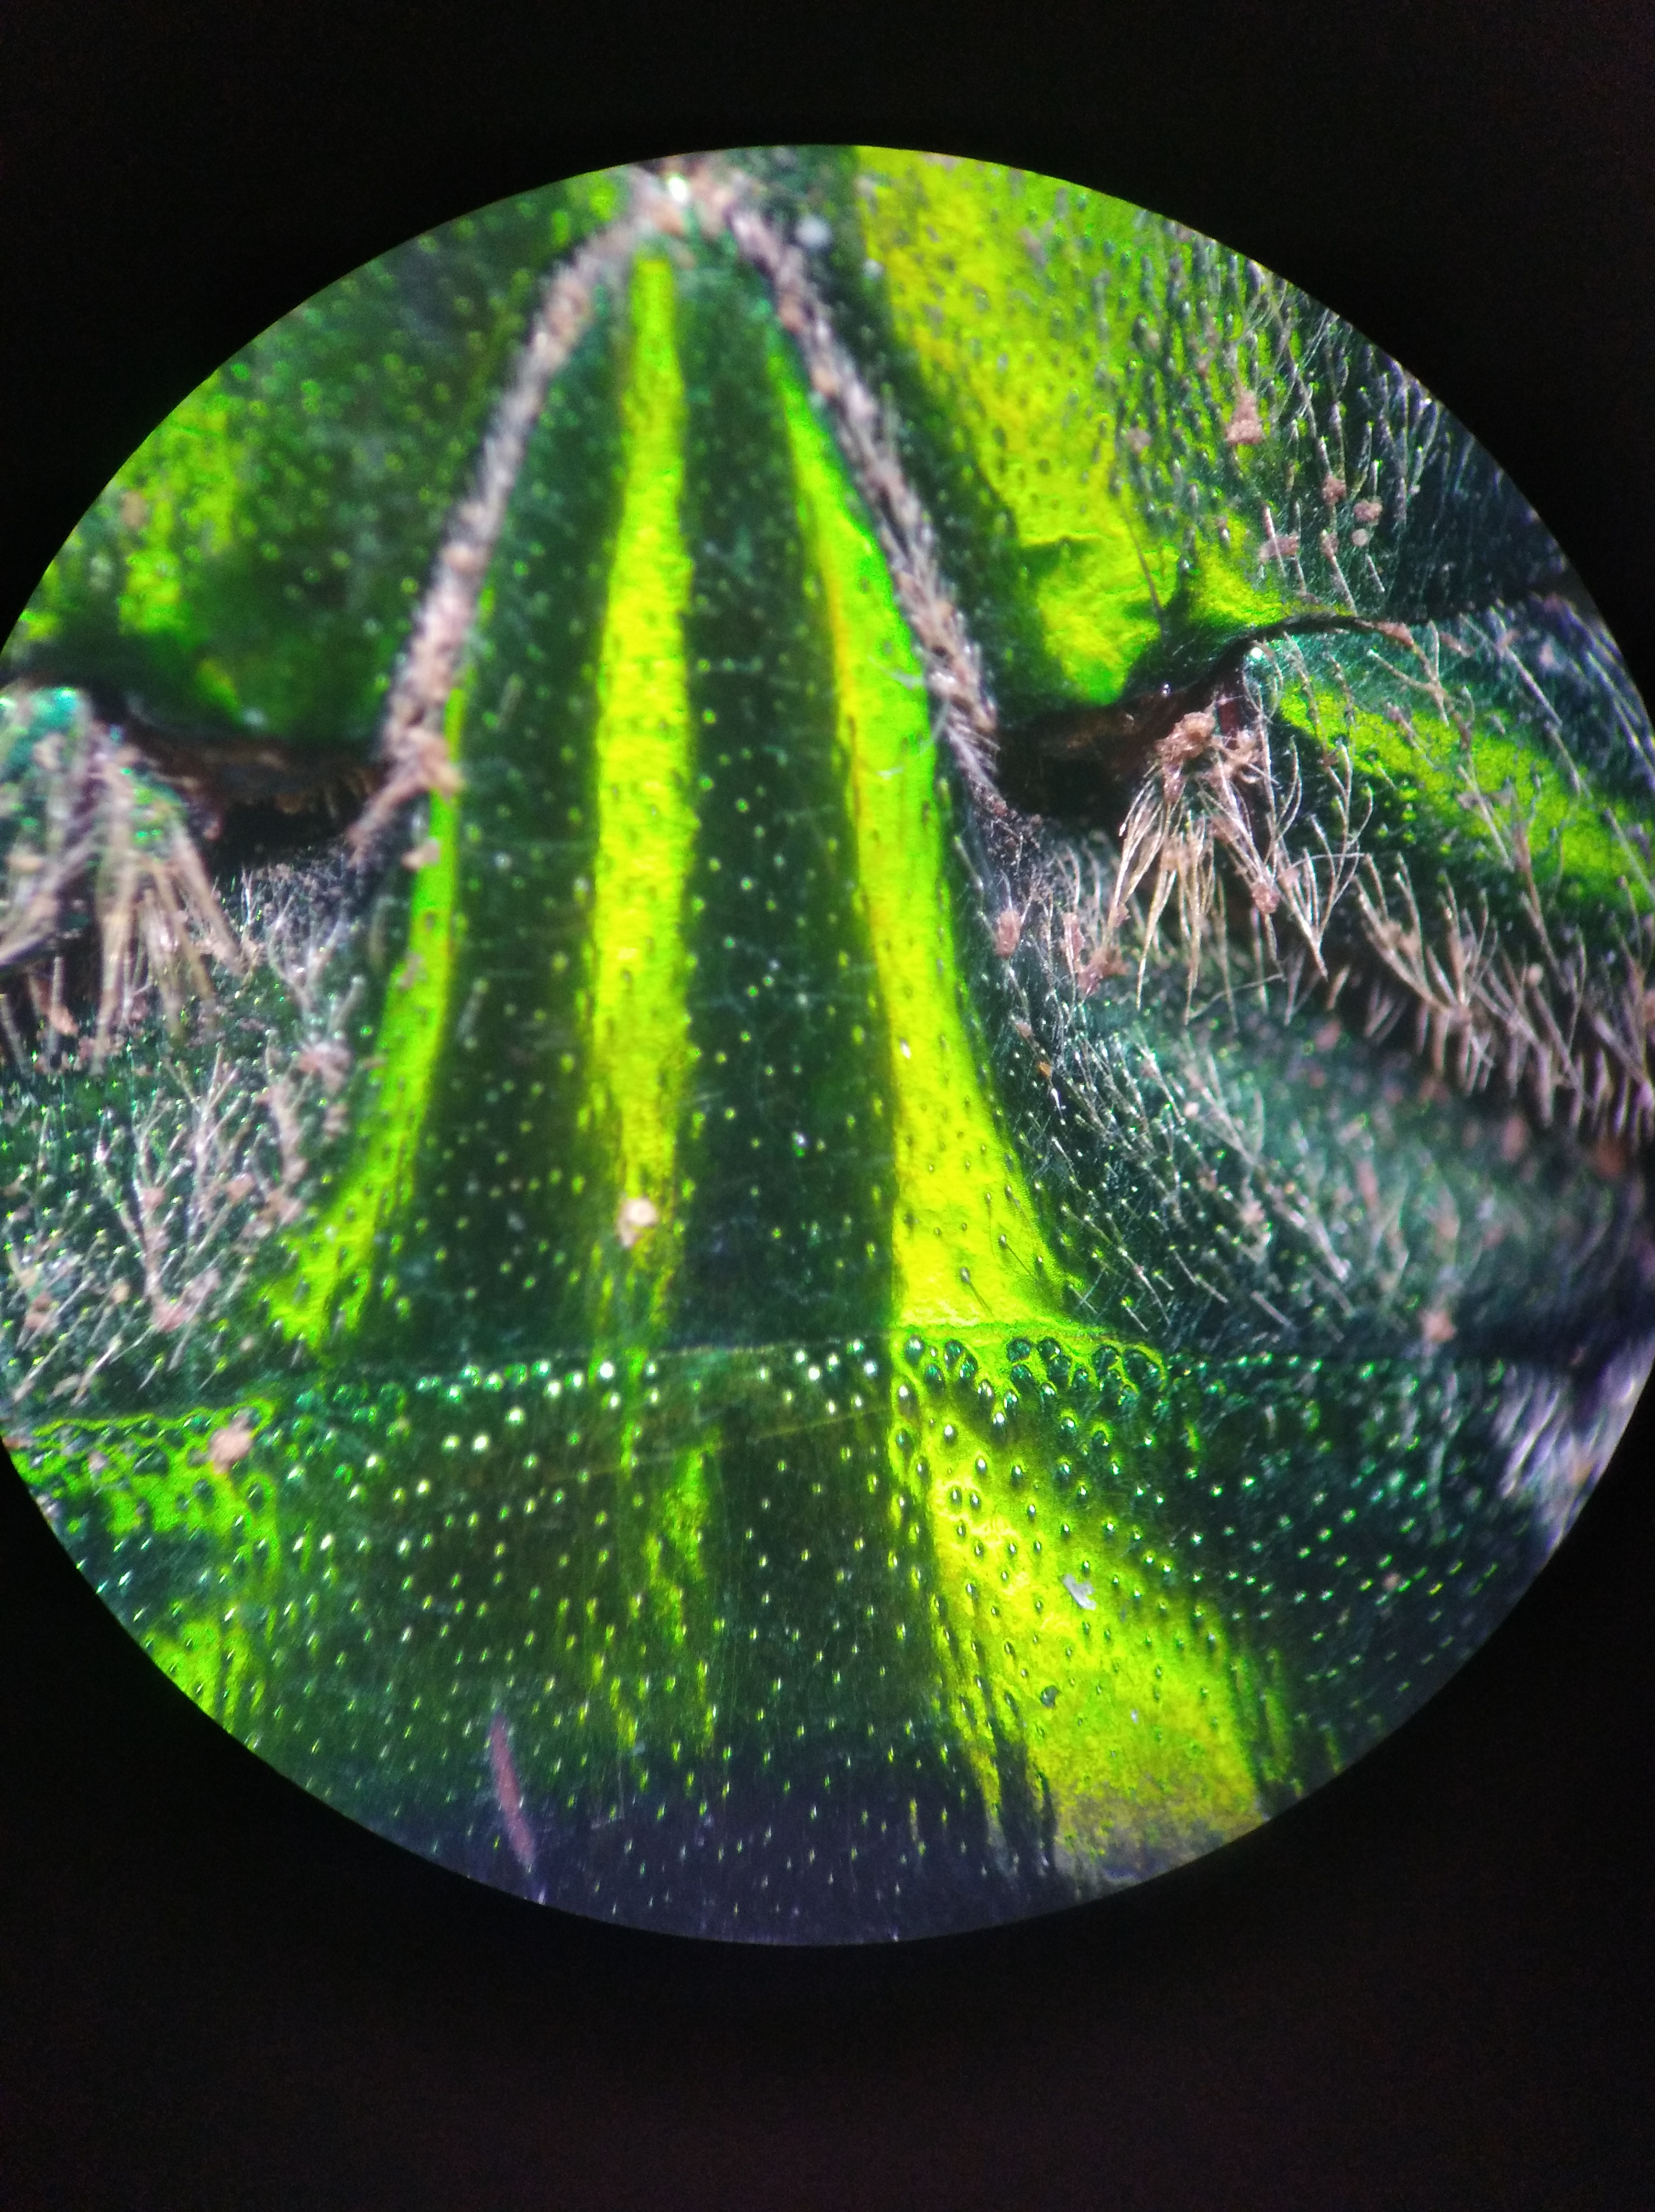
\includegraphics[width=0.25\textwidth]{insecto1_abajo.jpg}
    \caption{Zoom de la parte ventral  del Buprestidae tipo 1}
    \label{fig:my_label}
\end{figure}


\noindent Escarabajo: Buprestidae tipo 2


\begin{figure}[H]
    \centering
    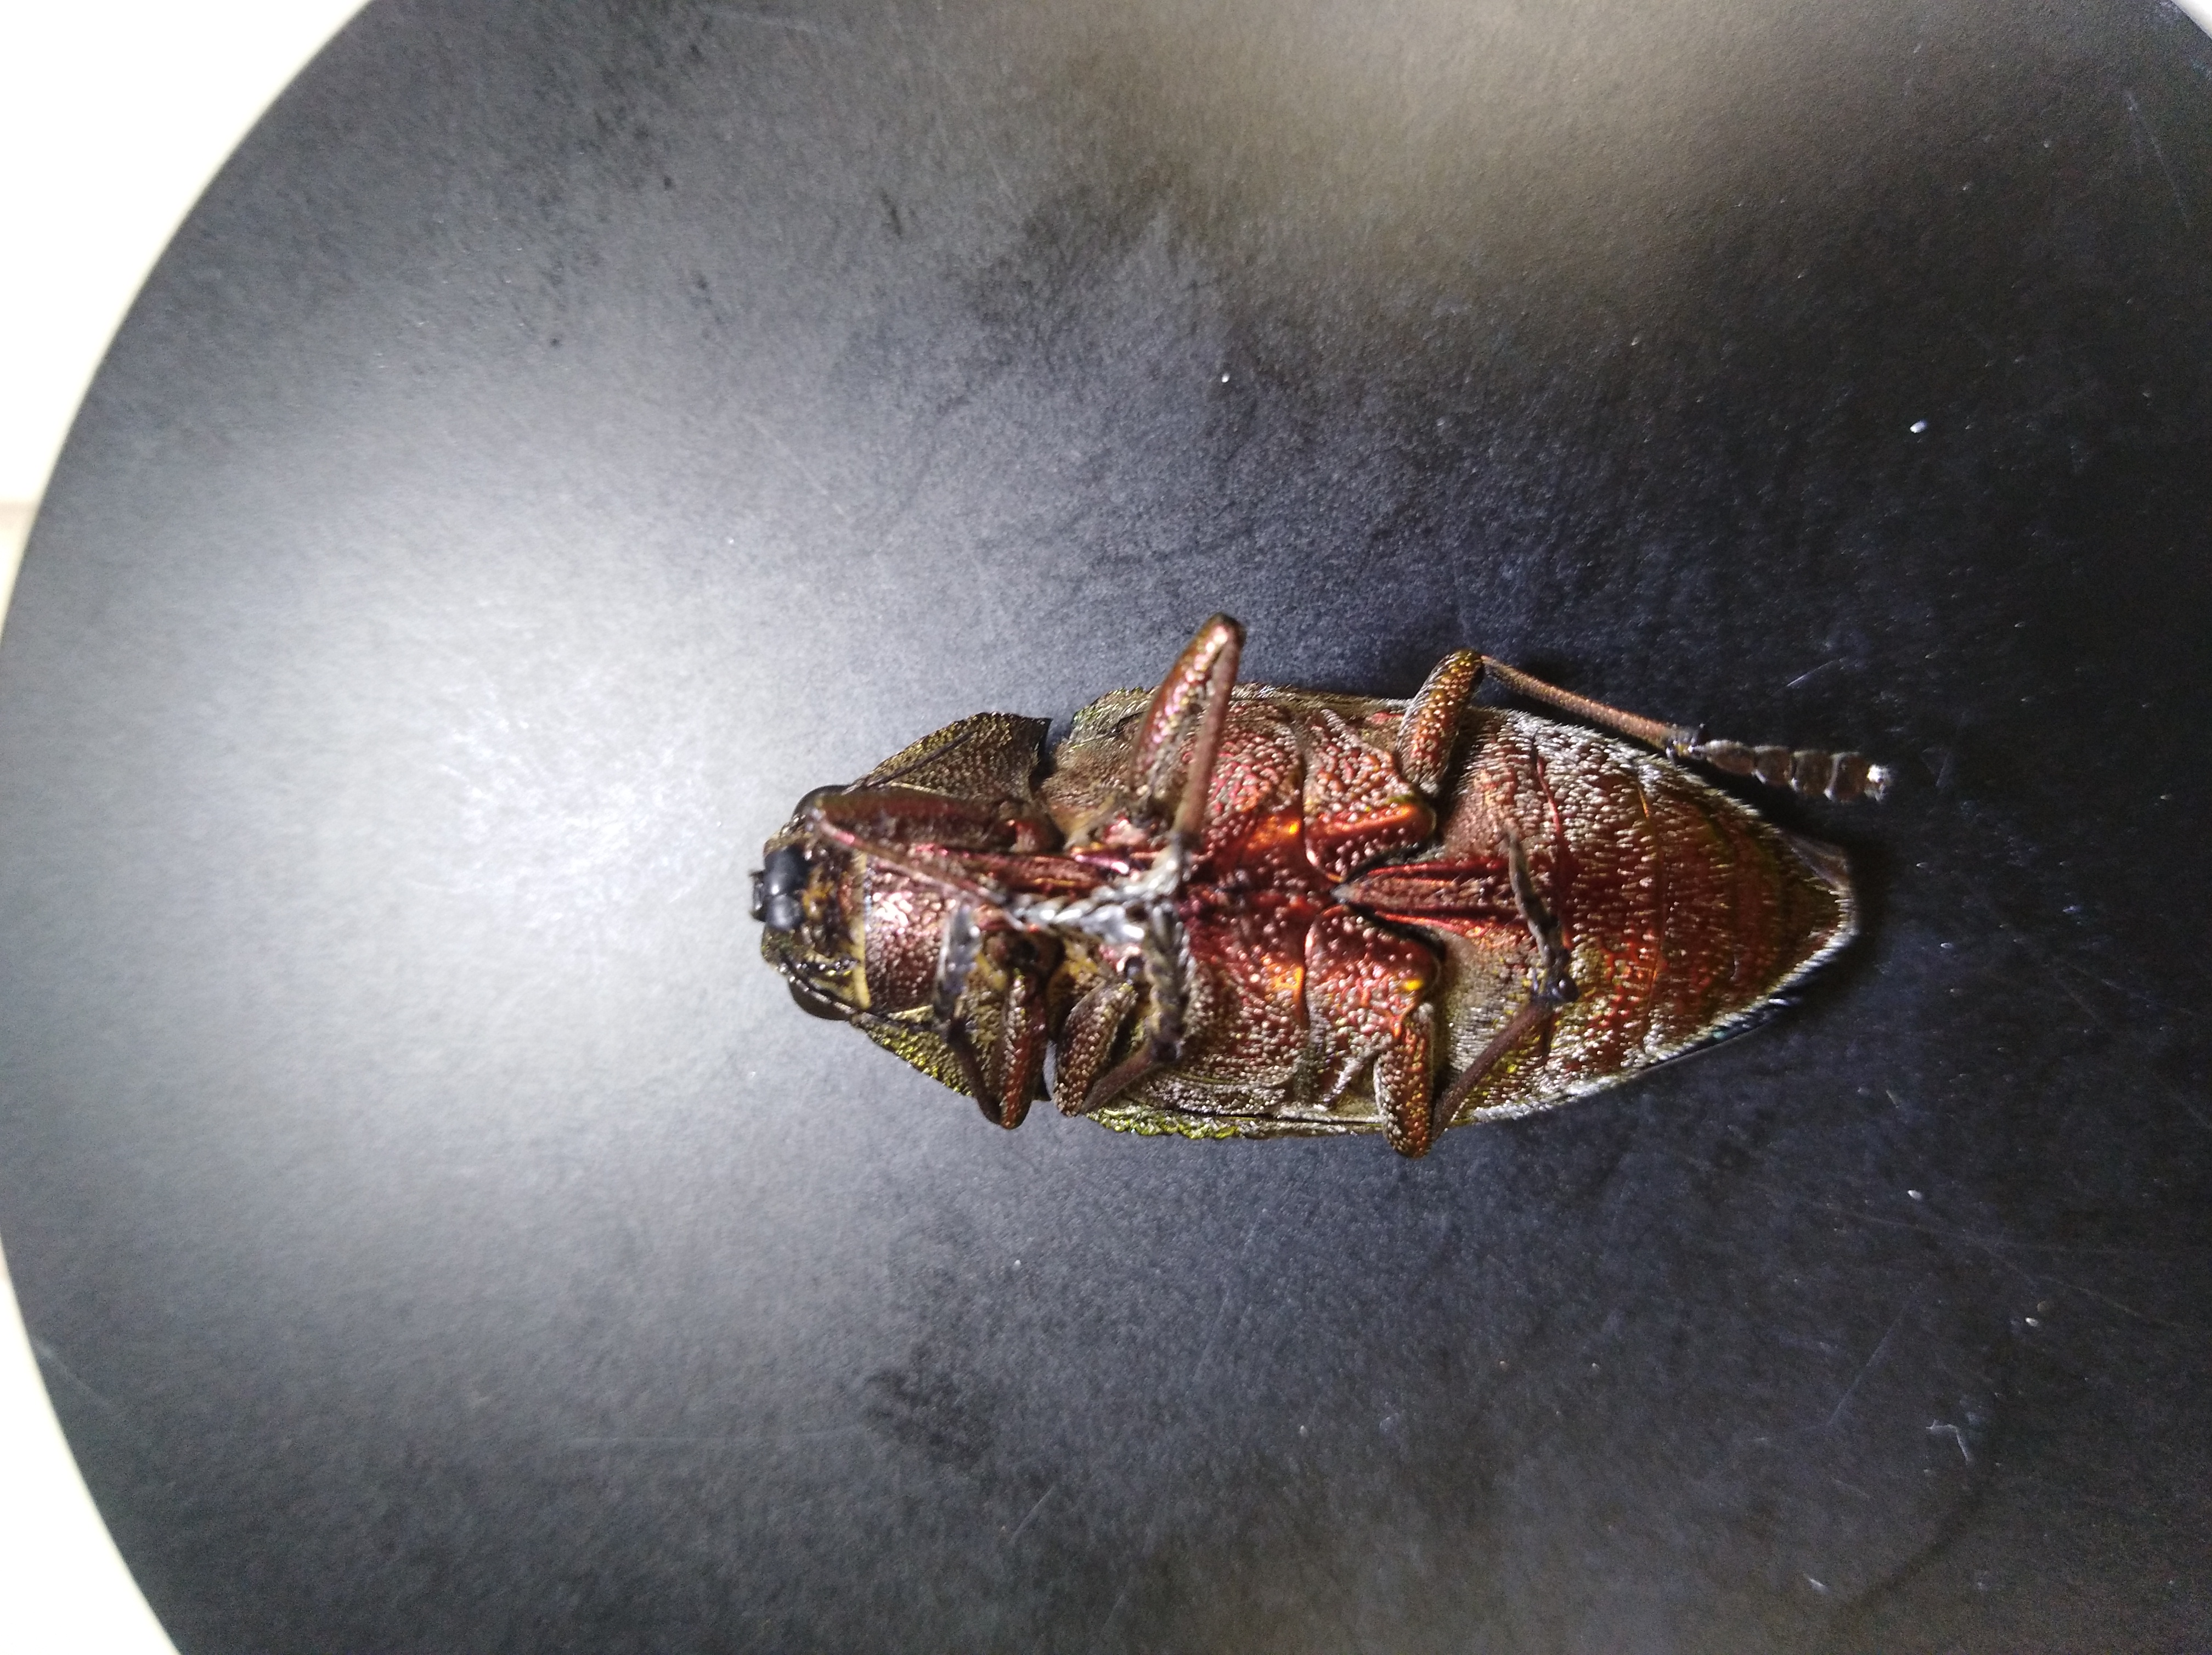
\includegraphics[width = 0.25\textwidth]{insecto2_ventral.jpg}
    \caption{insecto; Familia: Buprestidae}
    \label{tipos}
\end{figure}

\noindent Segundo escarabajo: Buprestidae tipo 2

\begin{figure}[H]
    \centering
    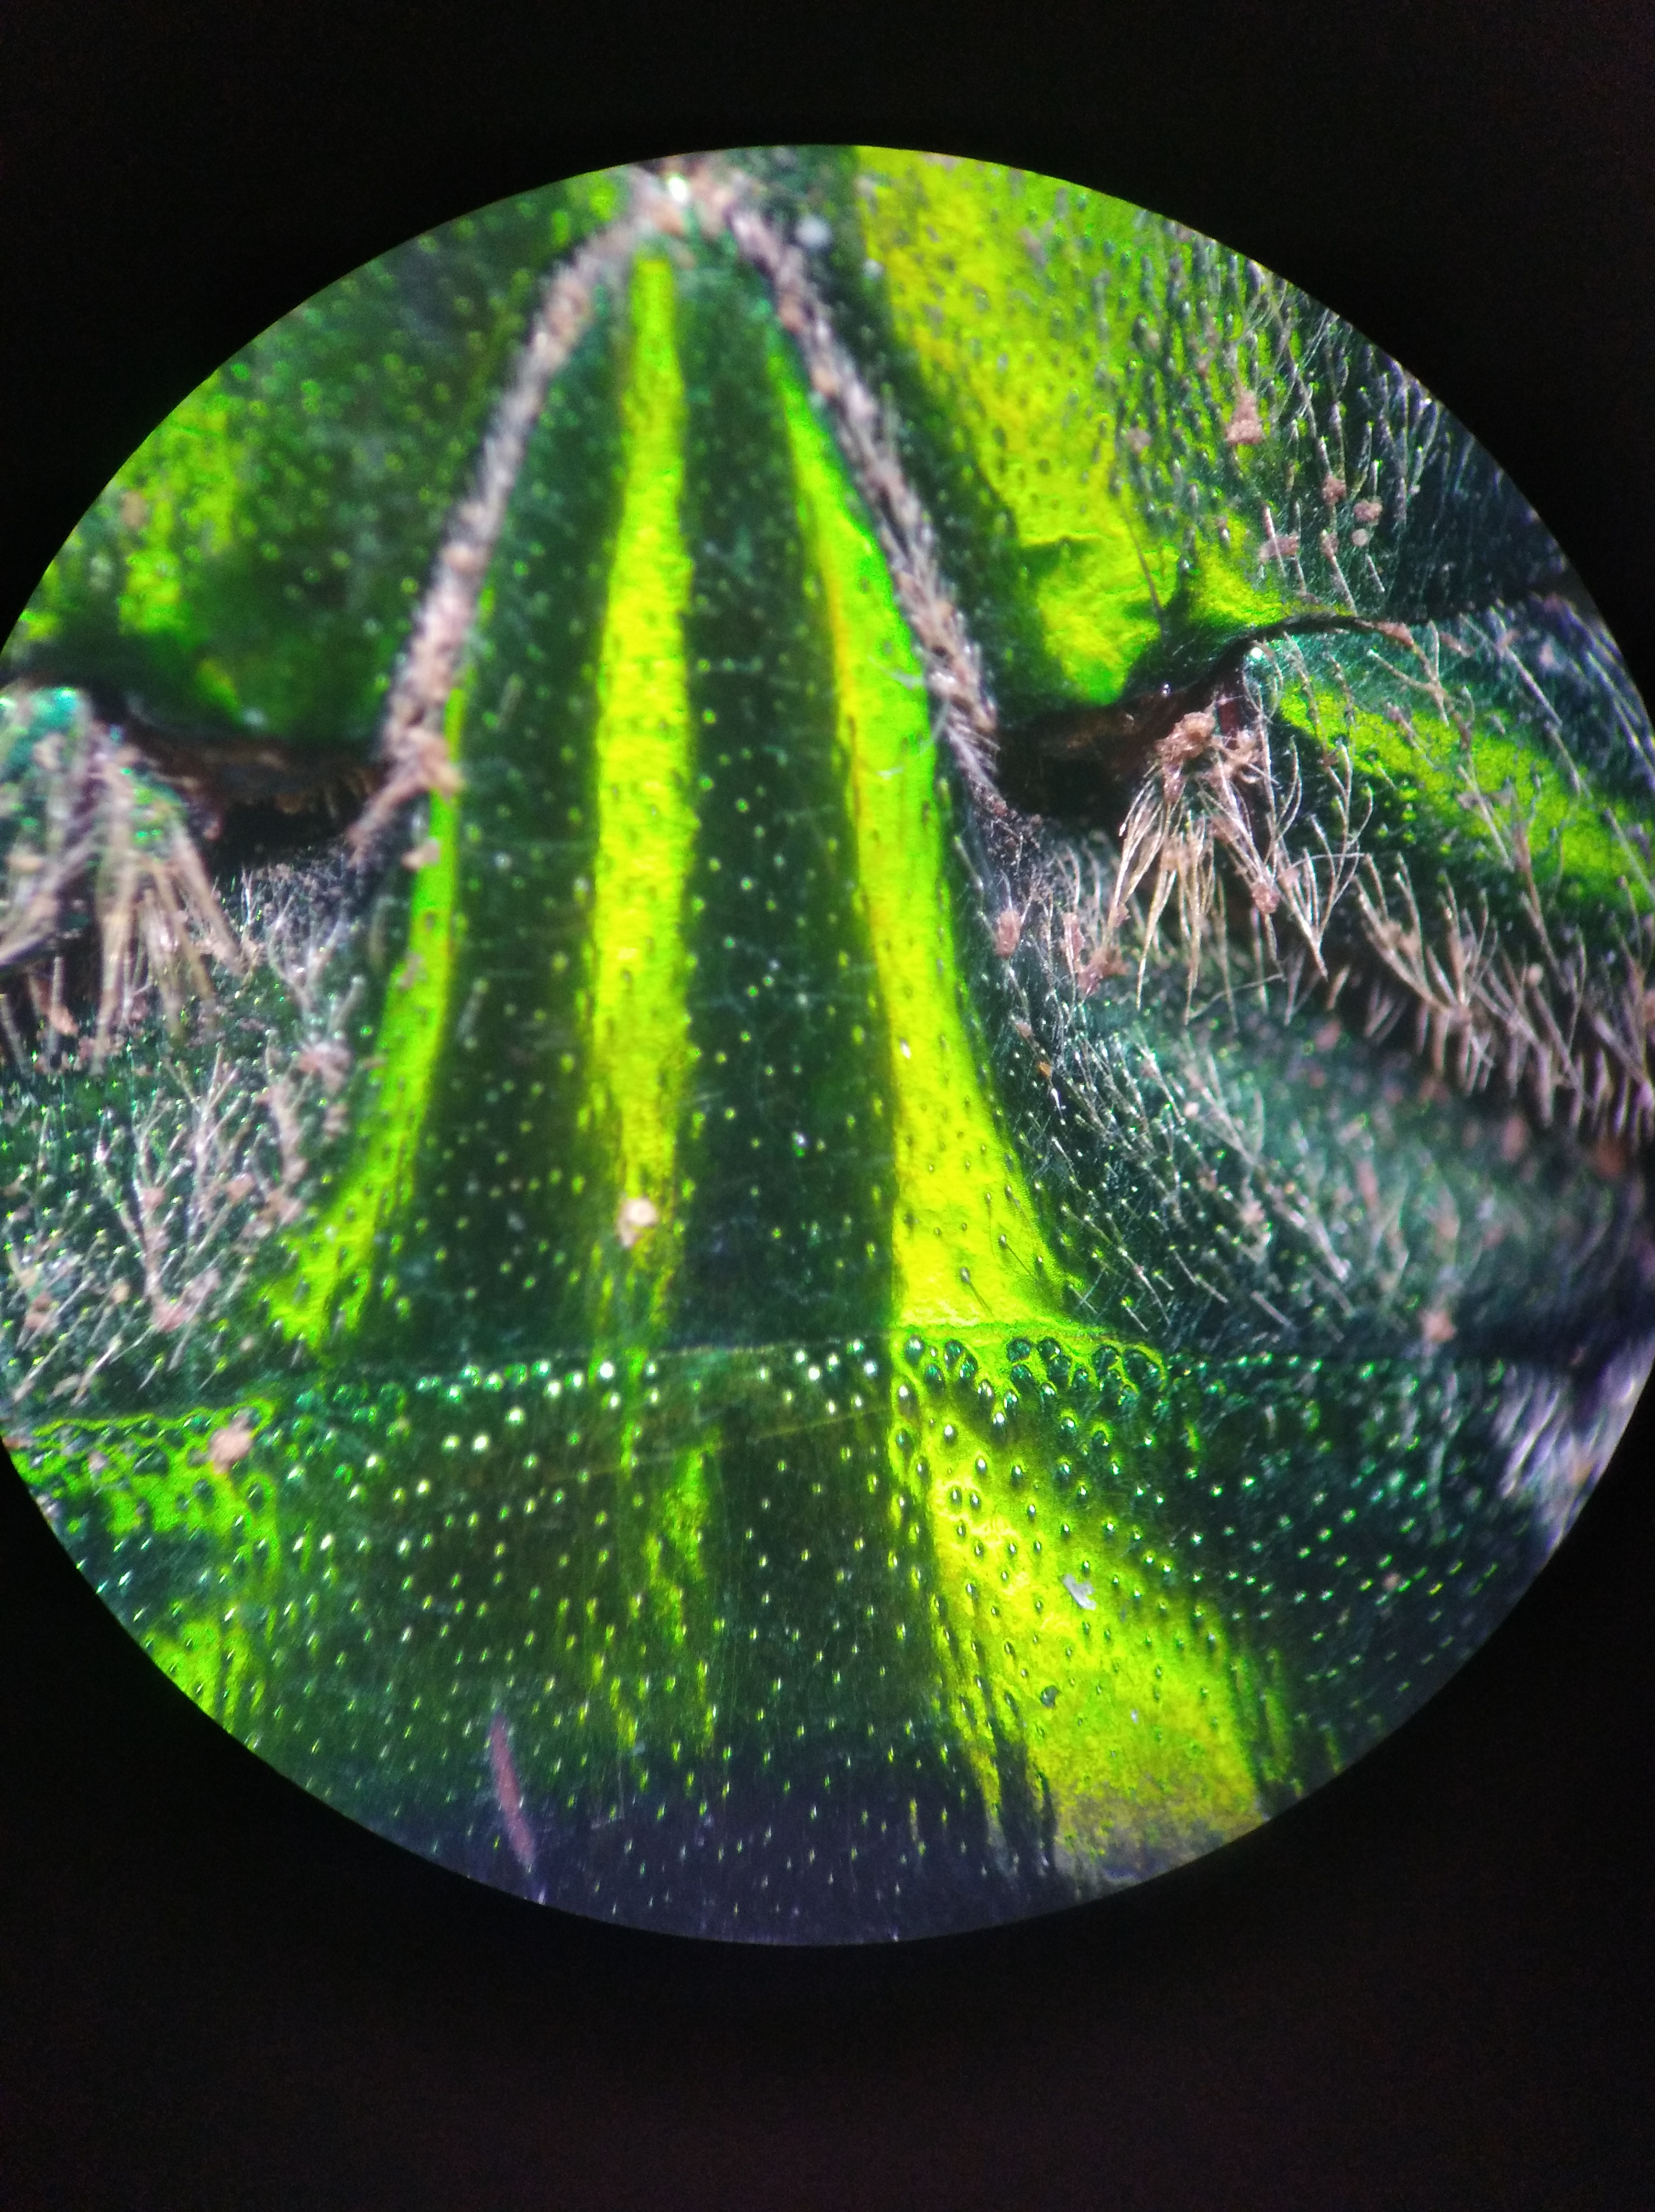
\includegraphics[width = 0.25\textwidth]{insecto1_abajo.jpg}
    \caption{Inseto, Buprestidae tipo 2}
    \label{tipos}
\end{figure}
 
\noindent Último insecto estudiado: La cigarra

\begin{figure}[H]
    \centering
    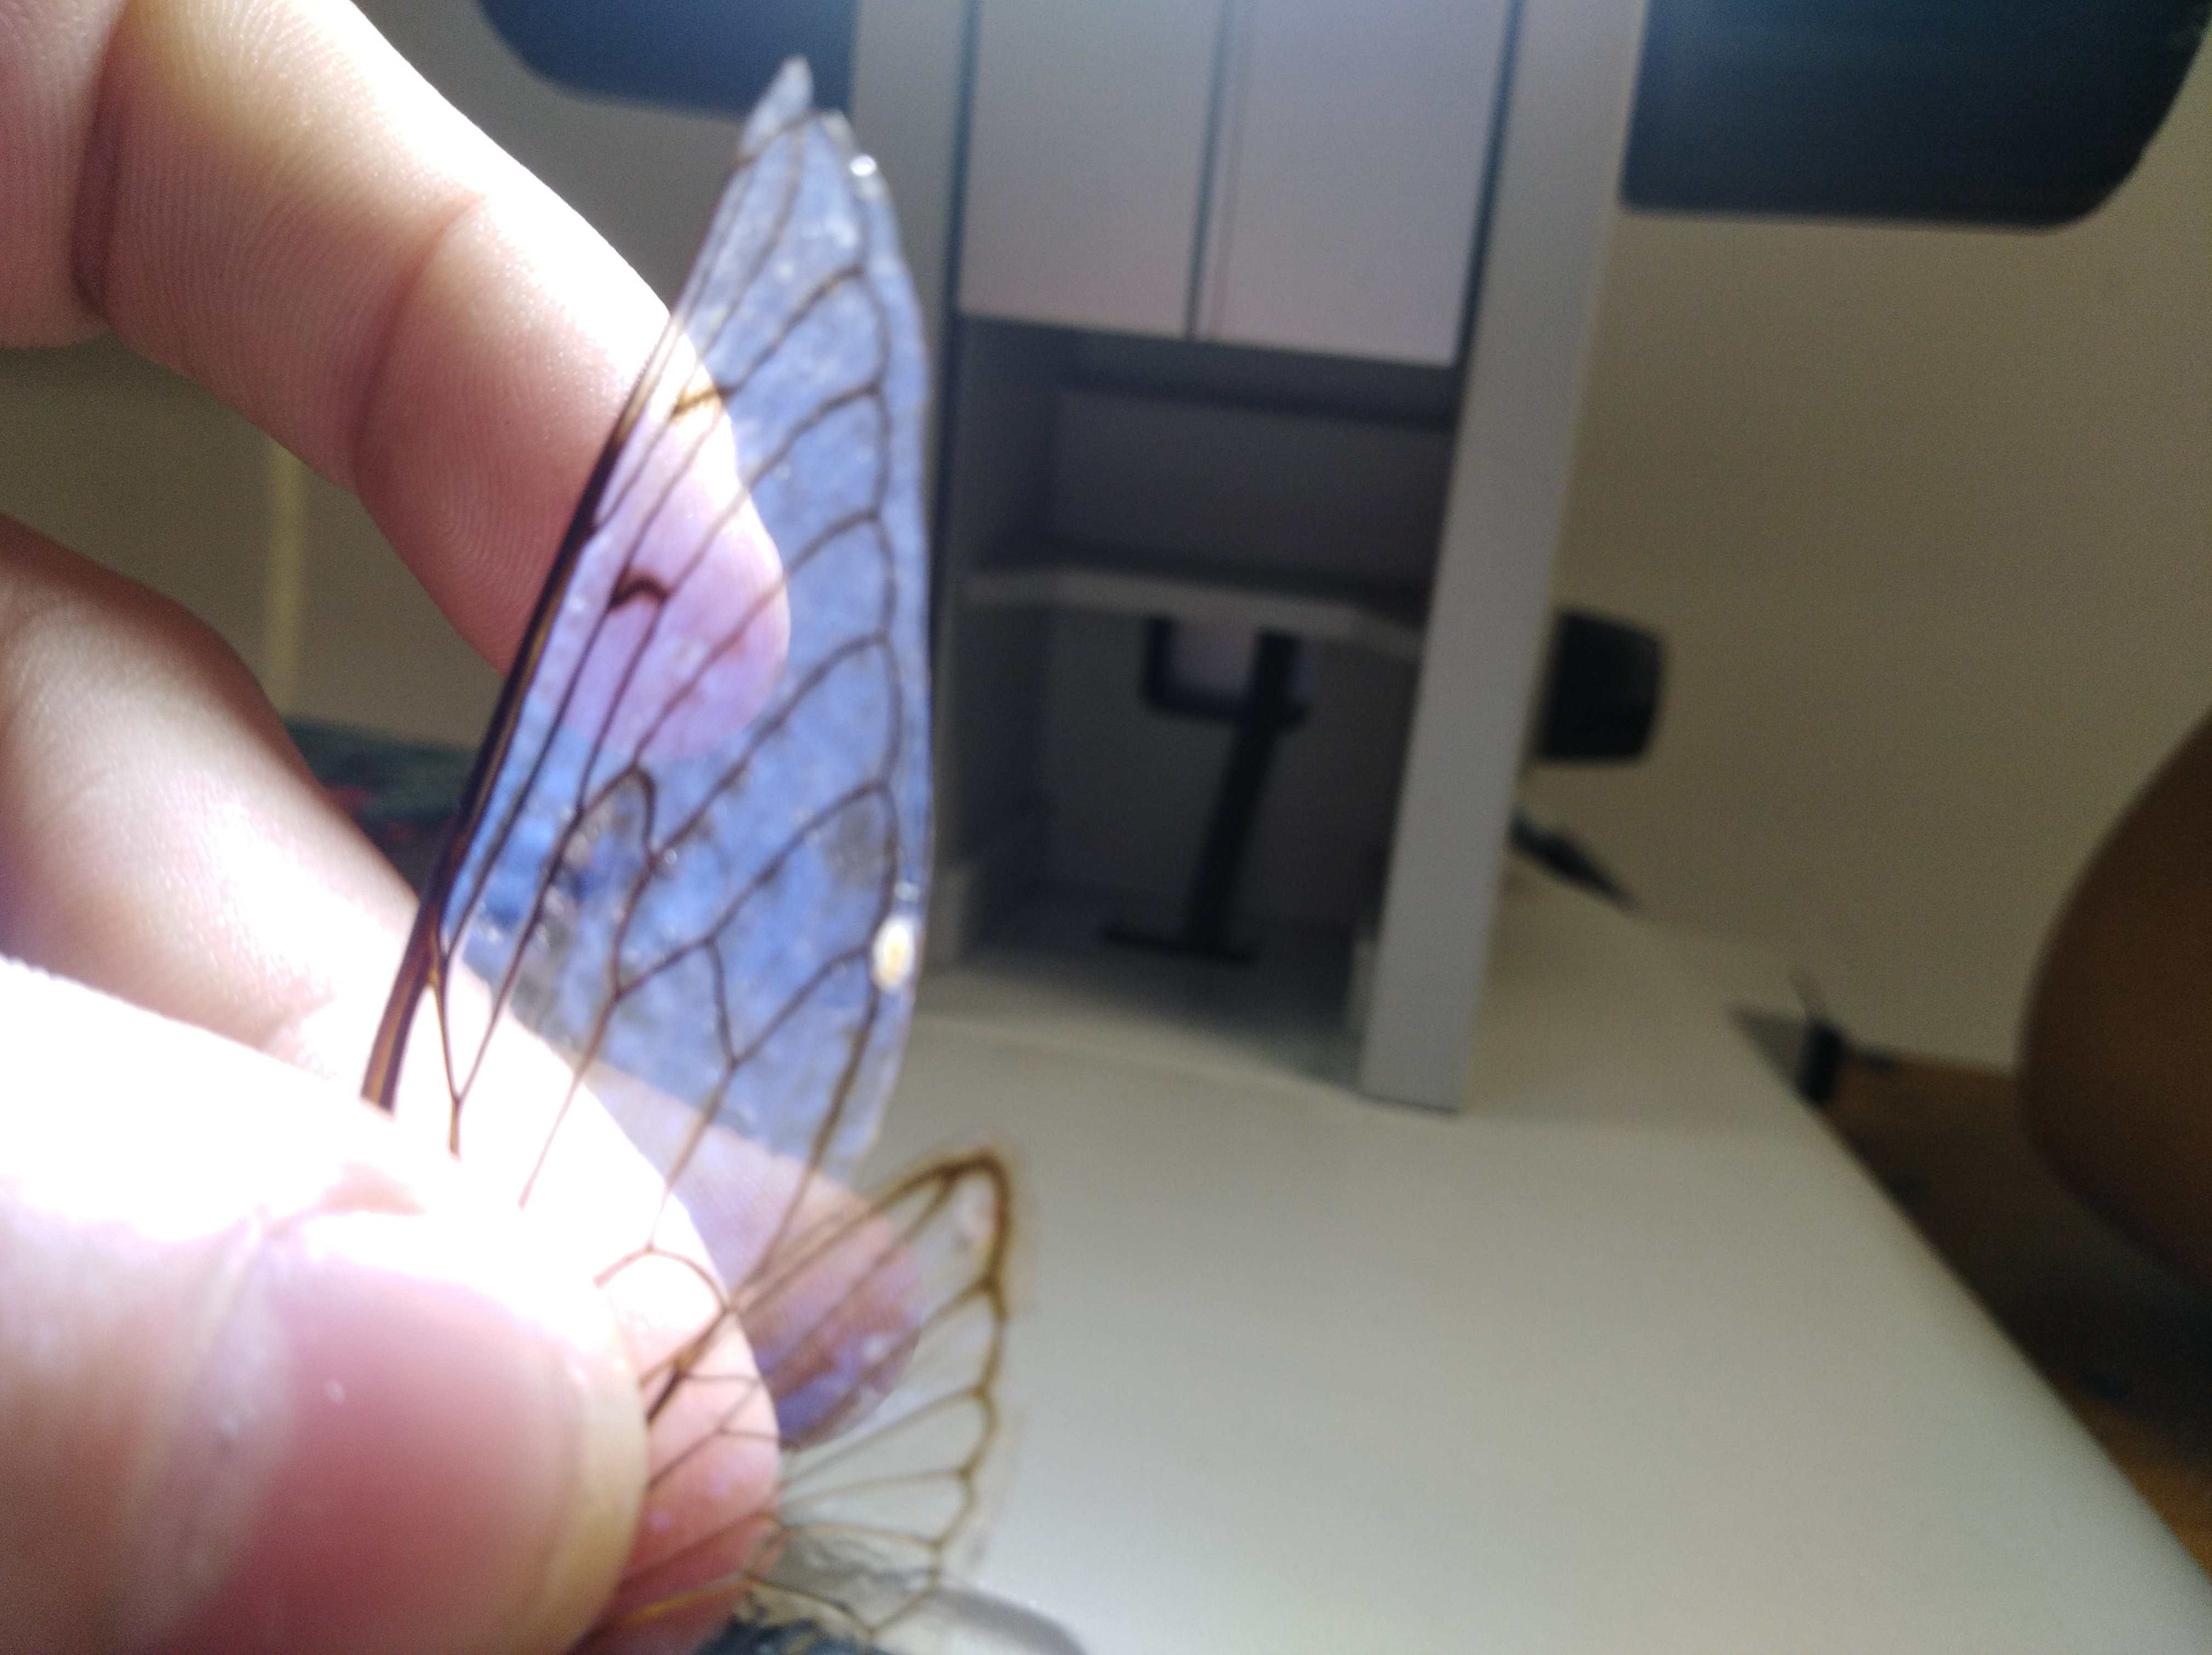
\includegraphics[width = 0.3\textwidth]{ala_dedo.jpg}
    \caption{Ala de la cigarra sostenida por una mano humana}
    \label{tipos}
\end{figure}
 
 Adicionalmente:
 
 \begin{figure}[H]
    \centering
    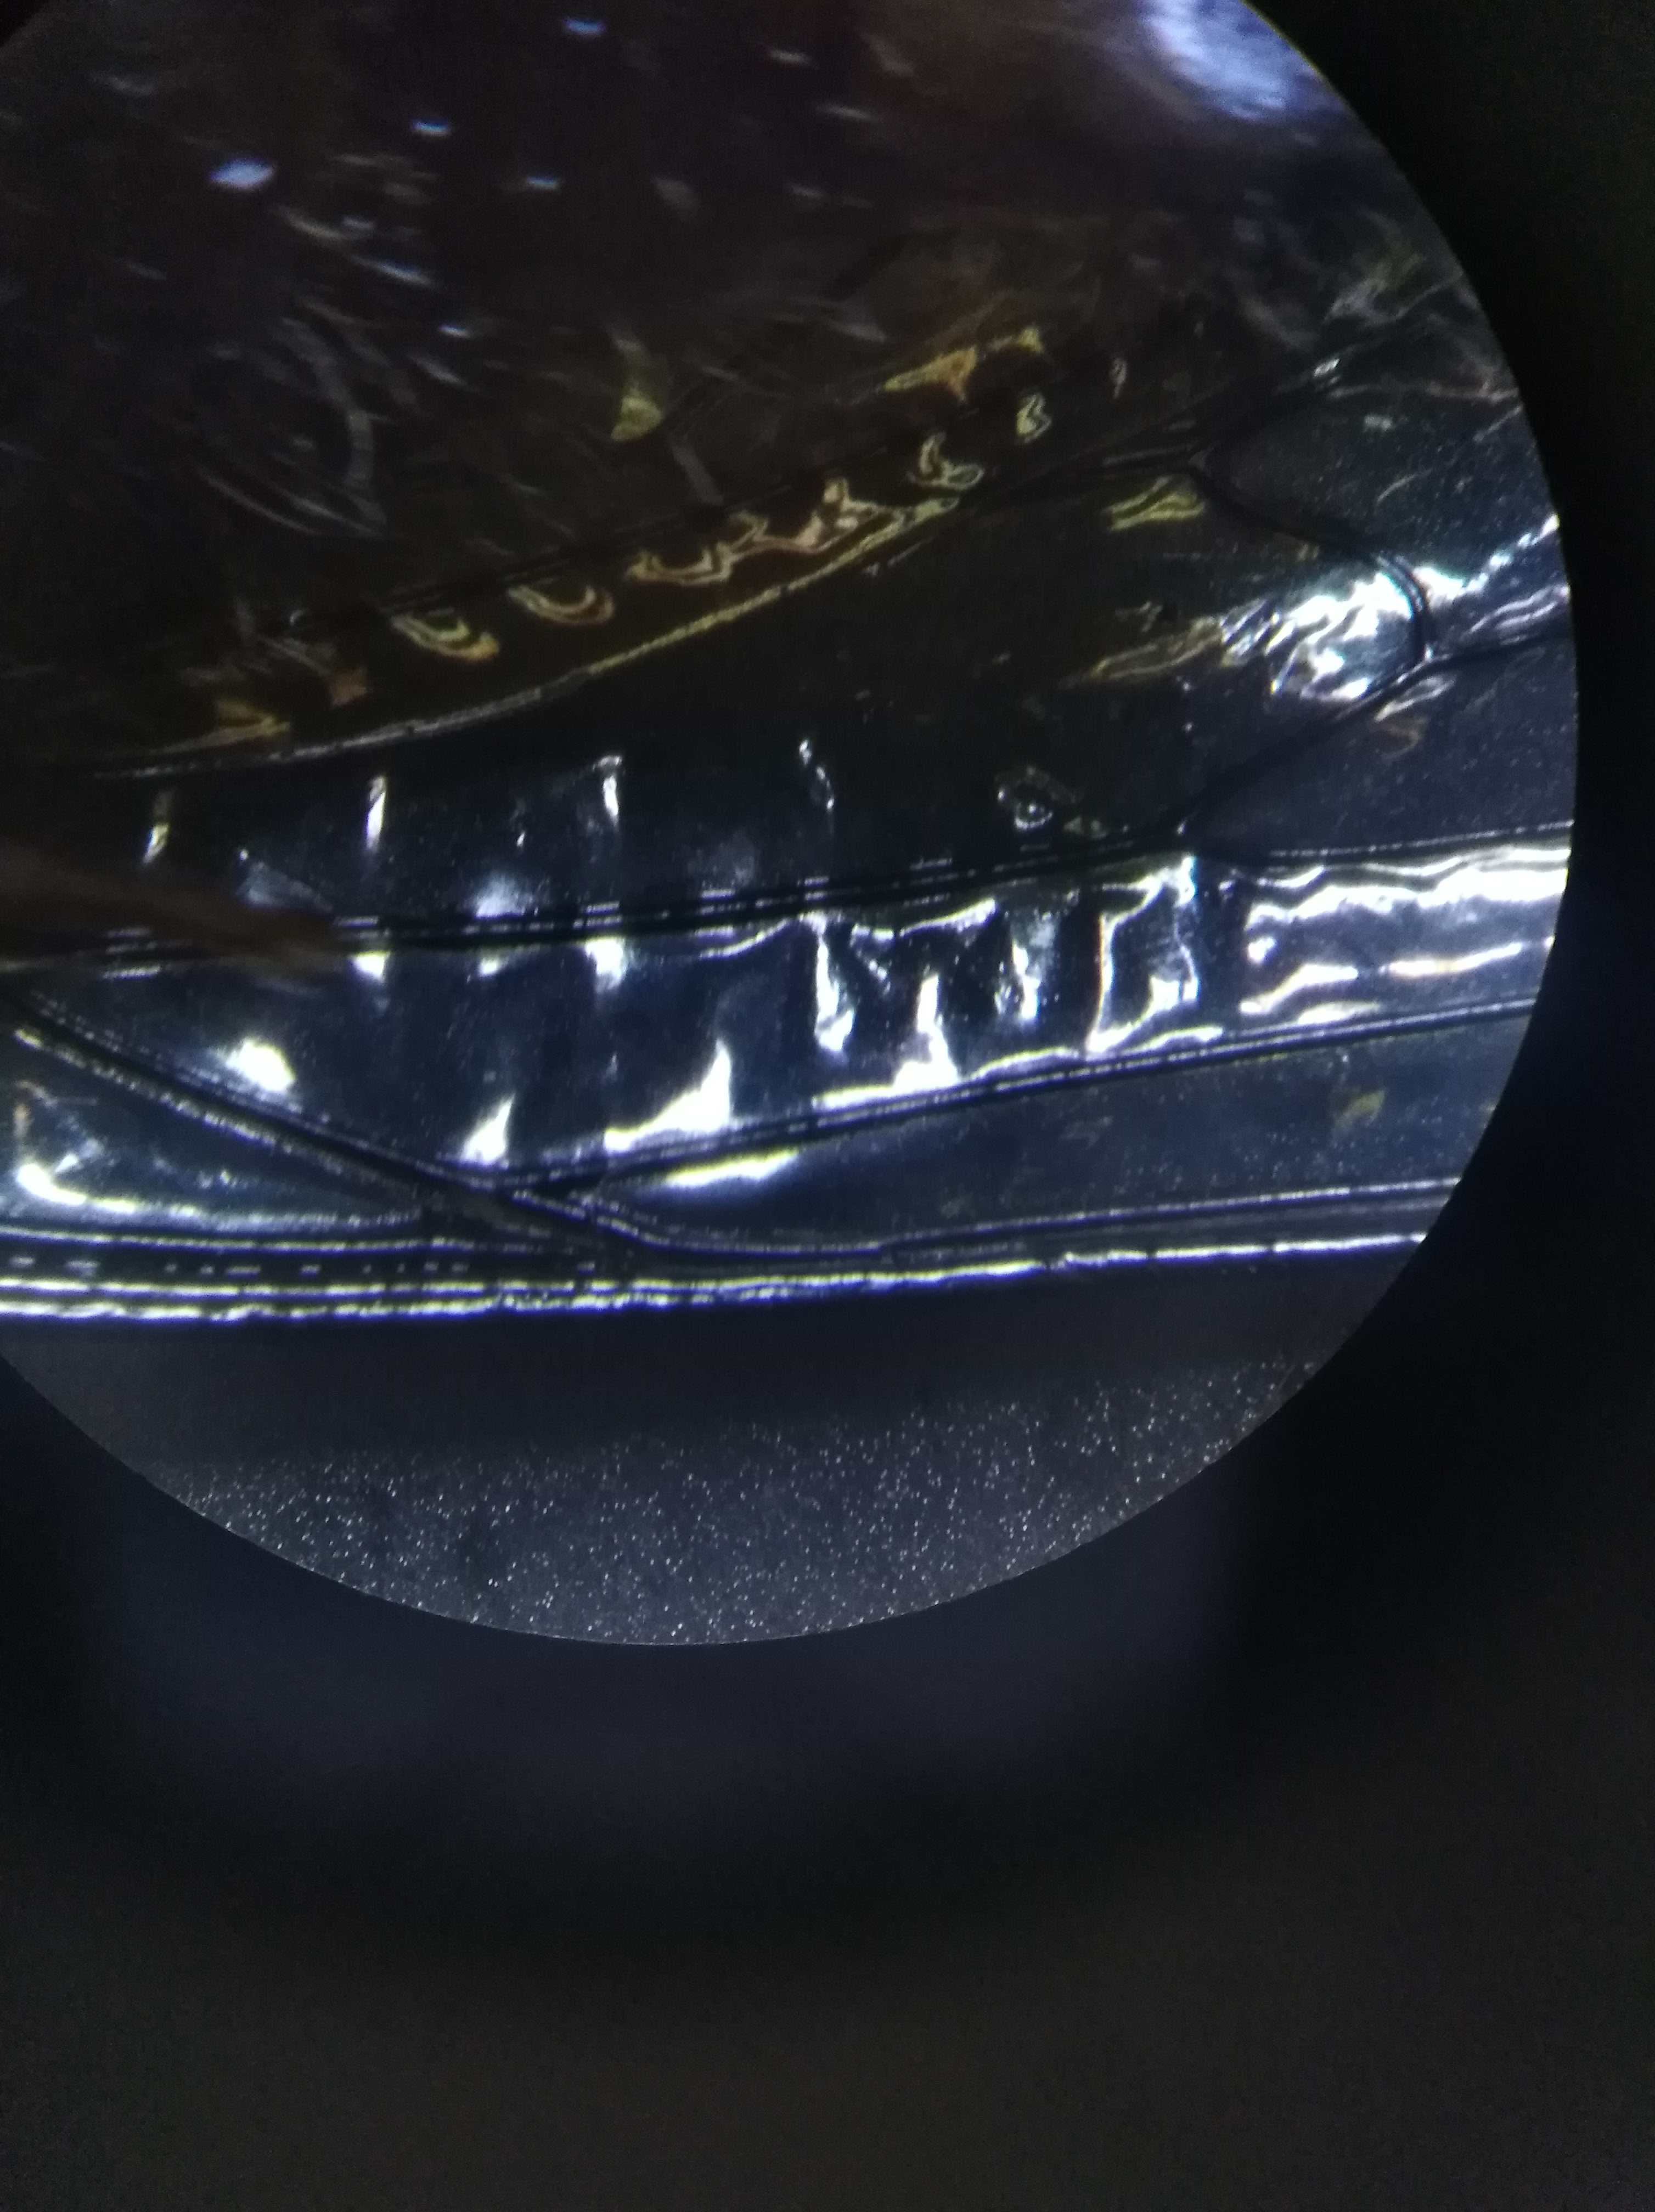
\includegraphics[width = 0.25\textwidth]{ala_cerca.jpg}
    \caption{Inseto, Buprestidae tipo 2}
    \label{tipos}
\end{figure}

\begin{figure}[H]
    \centering
    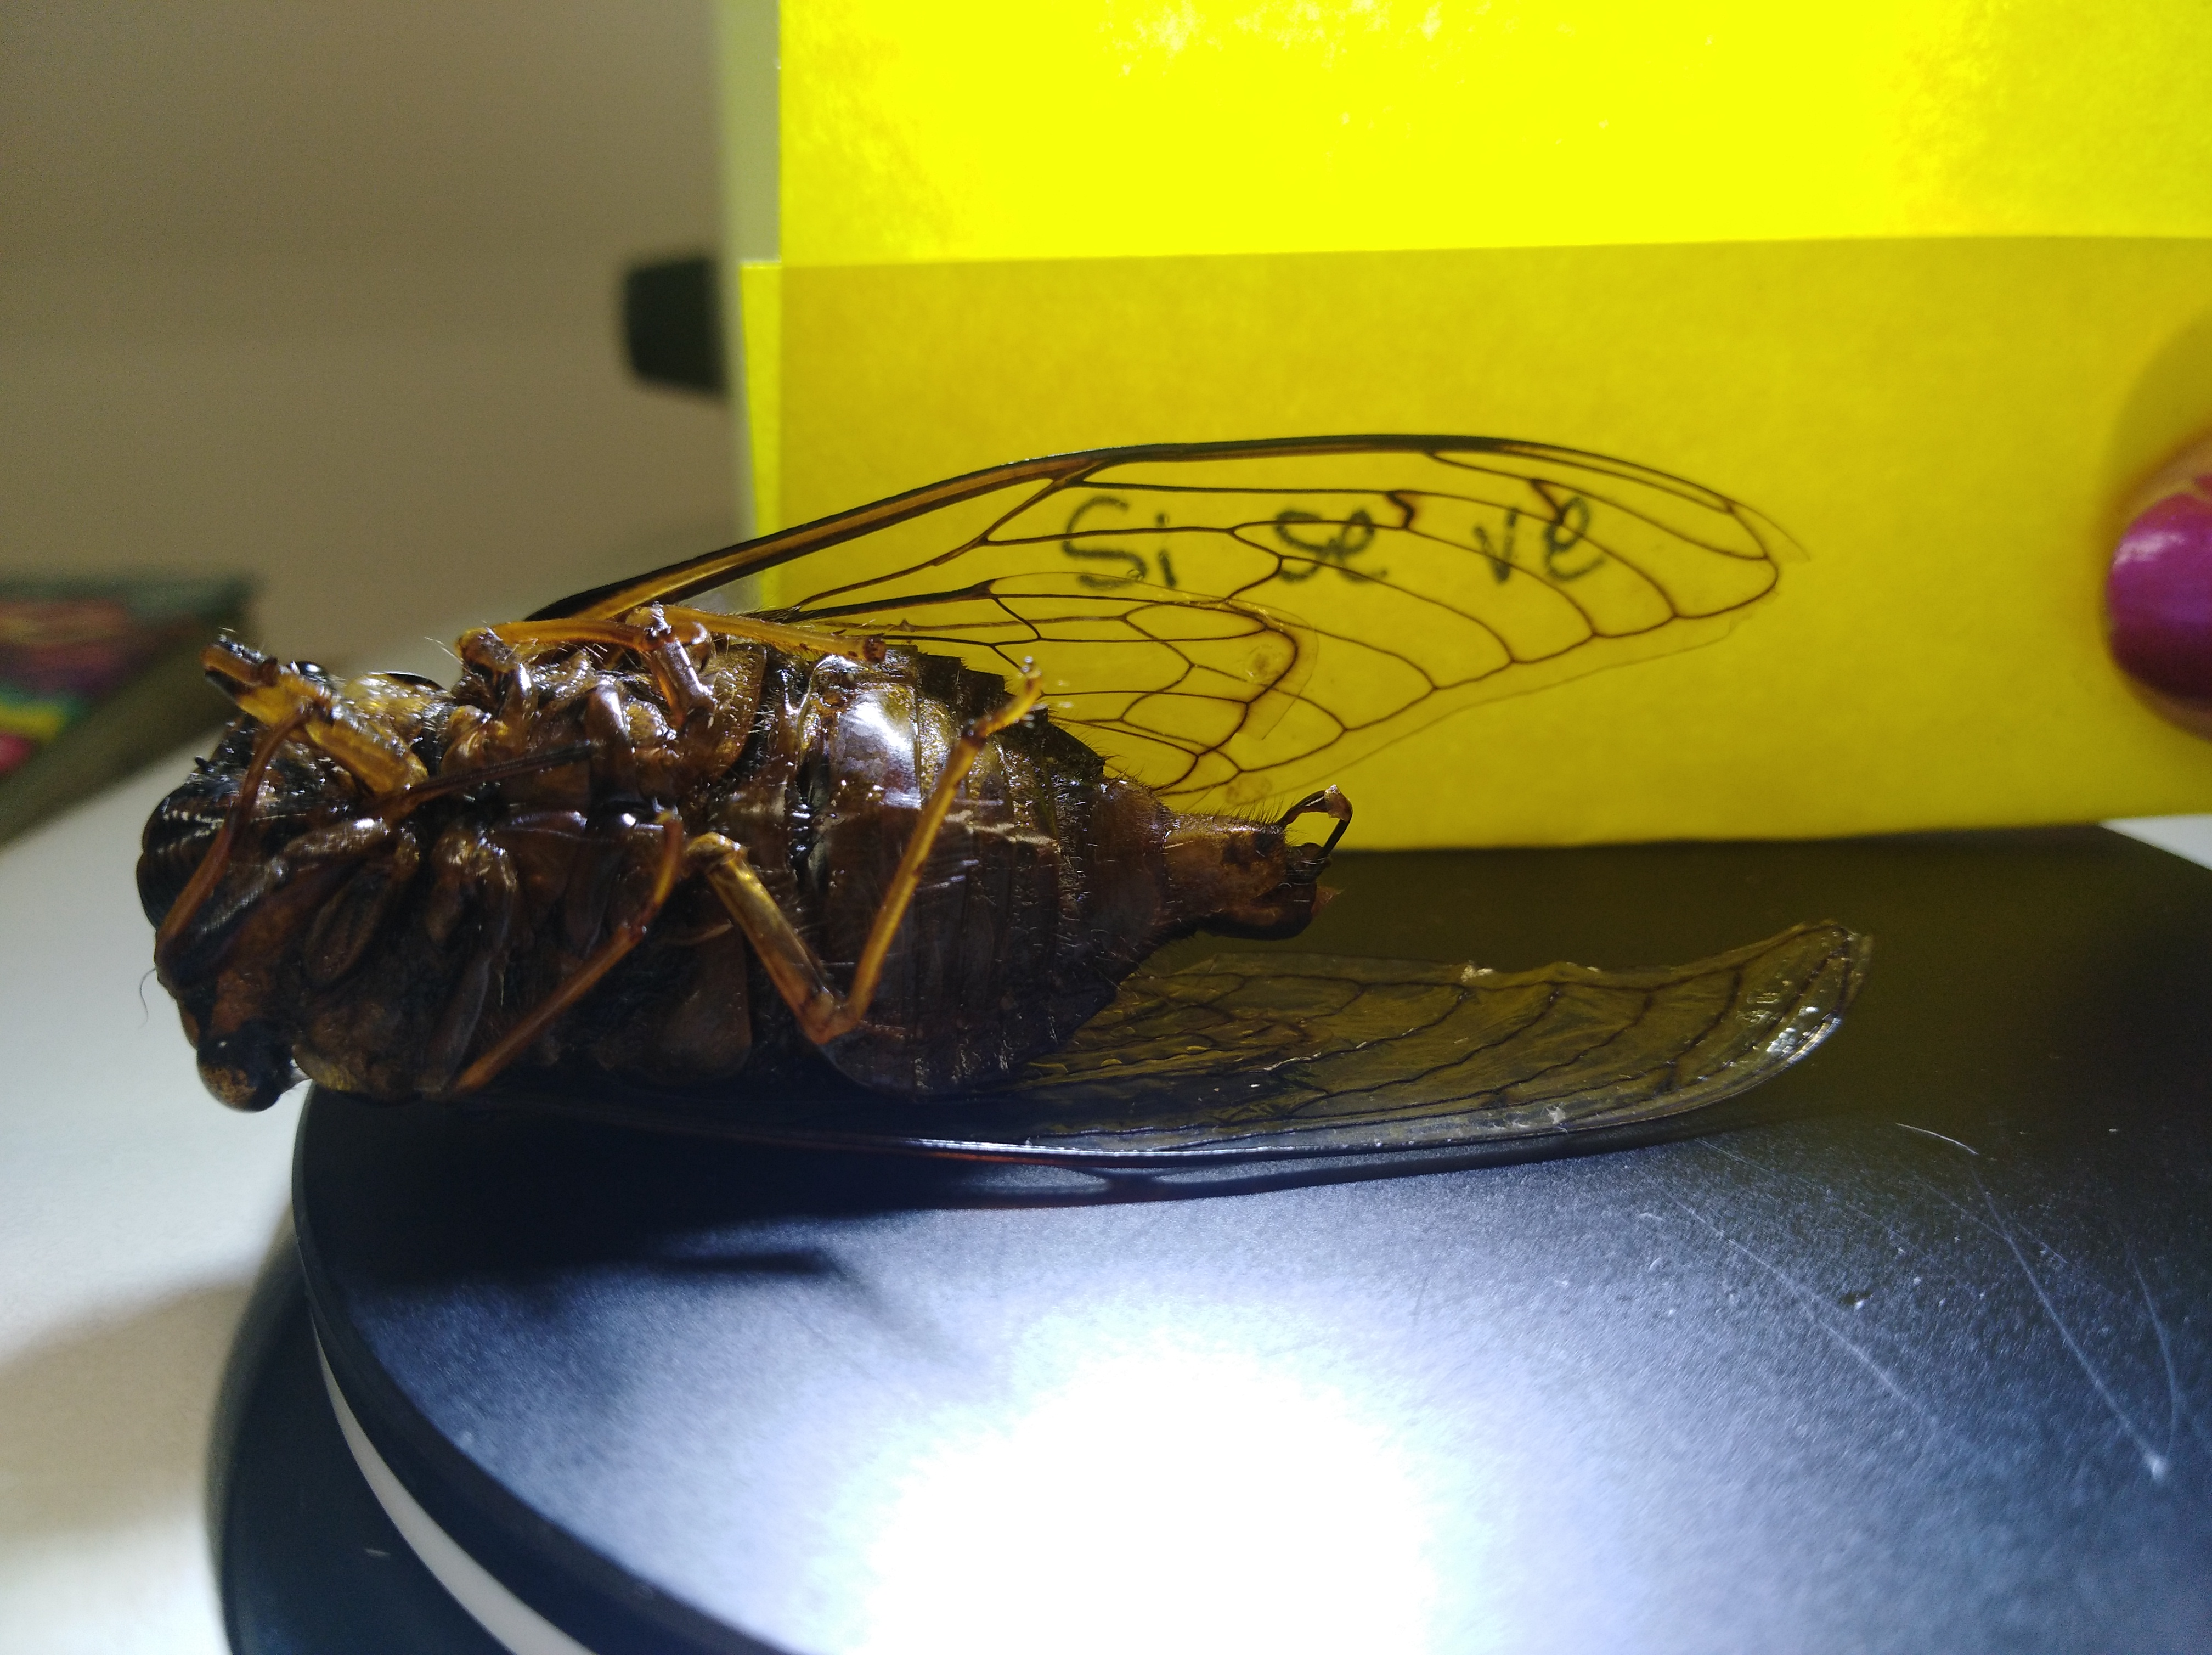
\includegraphics[width = 0.25\textwidth]{IMG_20190828_154520.jpg}
    \caption{Inseto, Buprestidae tipo 2}
    \label{tipos}
\end{figure}

\section*{Discusión de resultados}

Las fotografias tomadas muestran las texturas presentes en los exoesqueletos  de los diferentes insectos observados. En la superficie de la abeja se evidencia una estructura de escamas. Este tipo de estructuras son representativas en las alas de las mariposas Morpho Rethenor, cuya irisdicencia es atribuida a los arreglos de escamas los cuales se comportan como un metamaterial.  Aplicaciones directas con metalentes no se evidencian, sin embargo, estos insectos muestran caracteristicas muy importantes a nivel de metamateriales. La buprestidae tipo 2, o la cigarra, puede ser lo más cercano a un metalente, ya sus alas presentan iridiscencia por los diferentes arreglos en su superficie, y permite el paso de la luz. En la referencia \cite{dushkina2017coloration} se hace un estudio completo para este tipo de alas. Allí las iridiscencia azul a grandes ángulos de visión son producto de la dispersión altamente coherente desde láminas inclinadas y superpuestas en la escala de las crestas de las alas\cite{dushkina2017coloration}.

\section*{Conclusiones}

\begin{itemize}
    \item Con la realización de este estudio, se pudo mostar que en algunas especies, tales como Buprestidae y apidae, se presenta el fenómeno de iridiscencia debido a la estructura de su exoesqueleto, esto permite ver que dependiendo del ángulo con el que sea observado, se verá una tonalidad diferente.
    
    \item La micro estructura de los insectos más adecuada podrían ser la alas de las cigarra ya que, además de reflejar la luz en cierta tonalidad, permite el paso de la luz desde su interior, haciendo posible ver através de su ala.
    
    \item No en todas las especies estudiadas se pueden tomar como un metalente, ya que no cumple con todas las propiedades de esta requiere. Sin embargo, aquellos que no cumplen para metalente, podrían hacer su aporte como un metamaterial natural.
\end{itemize}

\printbibliography

\end{document}
